\section{Topological Validation of Midsurface}

Topological validation can be performed using two methods:
\begin{itemize}
[noitemsep,topsep=2pt,parsep=2pt,partopsep=2pt]
\item \textbf{Solid-to-Surface}: Find the relationship between the topological entities of a thin-solid and its corresponding Midsurface. Check whether the predicated Midsurface entities validate the non-manifold equation (\ref{eqn_nonmanifold}).
\item  \textbf{Surface-to-Solid}: Predict the topological entities of a possible thin-walled solid that could be generated by thickening of the given Midsurface.  These predicted entities can be validated against the entities of the original thin-solid as well as with the manifold equation (\ref{eqn_manifold}).
\end{itemize}

\todo[inline]{Reviewer B:  Poor figures.  All figures must have figure titles and be referred to by number in the main text. }

% ************* OLD FAILED ATTEMPT ********************************
%In the Thin wall manifold solid faces are classified as as $f_p$ (Principal-Main faces) and $f_t$ (Thickness or capping faces). Edges are classified as $e_p$ (Principal-Main edges) and $e_t$ (along thickness or capping edges). Vertices are classified as $v_t$ (thickness vertex) when they are connected to at-least one $e_t$ and $v_p$ (principal or radial vertex), when they are connected to only $e_p$s.
%
%\subsubsection{Steps: Topological dimension reduction}
%\begin{itemize}
%[noitemsep,topsep=2pt,parsep=2pt,partopsep=2pt,leftmargin=*]
%\item Given a manifold solid, half of the $f_p$s are retained in the corresponding midsurface. Thickness faces $f_t$s and edges $e_t$s are gone. 
%%\item {\em Genuses} are the holes and the {\em rings} in the midsurface
%\item Half of the thickness vertices $v_t$s will remain in the midsurface. But the difficulty comes in predicting vertices at the junctions (corresponding to $v_p$s). Additional information about radial group of  $v_p$s is not directly available in the solid model (unless loop traversal detects cycles). 
%\item For example, in case of {\em \bf L} shape, half the $v_p$s are present in the midsurface as radial vertices, but in case of {\em \bf T} shape thats not true. So the procedure which is valid for  junctions up to degree two, is not so for the higher degree junctions. Examples below demonstrate this.
%\item Expand the Solid equation (\ref{eqn_manifold}) to include newly defined faces, edges: $ (v_p + v_t) - (e_p  + e_t) + (f_p  + f_t) = 2 (s - g) + r$
%\item For midsurface of this Solid, number of topological entities are changed as follows:
%	\begin{itemize}
%	[noitemsep,topsep=2pt,parsep=2pt,partopsep=2pt,label={}, leftmargin=*]
%	\item $v_{nm} = (v_p + v_t)/2$
% 	\item $e_{nm} = e_p/2$
%  	\item $e_t  = f_t  = r = 0$
%  	\item $f_{nm} = f_p/2$
%  	\end{itemize}
%\item Validate if the non-manifold equation $v_{nm} - e+{nm} + f_{nm} == (s_{nm} - g_{nm}) $ is honored.
%\end{itemize}
%
%\subsubsection{Examples}
%\begin{itemize}
%[noitemsep,topsep=2pt,parsep=2pt,partopsep=2pt,leftmargin=*]
%\item For Simple plate:
%	\begin{itemize}
%	[noitemsep,topsep=2pt,parsep=2pt,partopsep=2pt,label={}, leftmargin=*]
%%	\item \textcolor{blue}{``picture of the plate''}
%	\item $f_p =2,f_t=4,e_p=8,e_t=4,v_t=8,v_p=0,s=1,g=0$
% 	\item $v_{nm} = (v_t + v_p)/2 = 8 /2 = 4$
%  	\item $e_{nm} = e_p/2 = 8/2 = 4$
%  	\item $f_{nm} = f_p/2 = 2/2 = 1$
%  	\item $s_{nm} = 1, g_{nm} = 0$
%  	\item $v_{nm} - e_{nm} + f_{nm} = 4 - 4 +1 = 1 = (s_{nm} - g_{nm})$.
%  	\item \textbf{Result}: \textcolor{green}{Valid}
%  	\end{itemize}
%
%\item For 'L' shaped plate:
%	\begin{itemize}
%	[noitemsep,topsep=2pt,parsep=2pt,partopsep=2pt,label={}, leftmargin=*]
%%	\item \textcolor{blue}{``picture of L''}
%	\item $f_p =4,f_t=4,e_p=14,e_t=4,v_t=8,v_p=4,s=1,g=0$
% 	\item $v_{nm} = (v_t + v_p)/2 = (8+4) /2 = 6$
%  	\item $e_{nm} = e_p/2 = 14/2 = 7$
%  	\item $f_{nm} = f_p/2 = 4/2 = 2$
%  	\item $s_{nm} = 1, g_{nm} = 0$
%  	\item $v_{nm} - e_{nm} + f_{nm} = 6 - 7 + 2= 1 = (s_{nm} - g_{nm})$.
%  	\item \textbf{Result}: \textcolor{green}{Valid}
%  	\end{itemize}
%  	
%  	\item For 'T' shaped plate: 
%	\begin{itemize}
%	[noitemsep,topsep=2pt,parsep=2pt,partopsep=2pt,label={}, leftmargin=*]
%%	\item \textcolor{blue}{``picture of T''}
%	\item $f_p =5,f_t=5,e_p=20,e_t=6,v_t=12,v_p=4,s=1,g=0$
% 	\item $v_{nm} = (v_t + v_p)/2 = (12+4) /2 = 8$
%  	\item $e_{nm} = e_p/2 = 20/2 = 10$
%  	\item \textcolor{red}{$f_{nm} = f_p/2 = 5/2 = 2.5$}
%  	\item $s_{nm} = 1, g_{nm} = 0$
%  	\item $v_{nm} - e_{nm} + f_{nm} = 6 - 7 + 2= 1 = (s_{nm} - g_{nm})$.
%  	\item \textbf{Result}: \textcolor{red}{Invalid}
%  	\end{itemize}
%
%\end{itemize}
%
%\textbf{Conclusion}: Manifold equation of Thin Solid cannot be simplistically converted to non-manifold equation of its midsurface. Thus this direction of validation has limitations. Following section examines if the other direction of validation is possible or not.


\subsection{Sheet Metal Solid to Midsurface Transformation}

Given a sheet metal solid, below is an approach to propose the dimension-reduction-transformation equations for predicting the topological entities of its corresponding midsurface. The given solid model is first decomposed into volumes and then the dimension-reduction-transformation is derived. Topology generated by the volumetric decomposition is called {\em Cellular Topology}.  Many commercial as well as academic methods are available for Cellular-Volumetric decomposition \cite{Woo2002, Woo2003, Chong2004, Cao2011,  Boussuge2013,  Boussuge2013a, Kim2014}. 

\todo[inline]{ In section 2.1 please expand the explanation of the cellular- 
volumetric decomposition method used and the result obtained for 
the case study part. In the context of sheet metal parts is it 
possible to obtain a cell with dimensionality 0 or 1? }
\todo[inline]{ In section 2.1 improve the figure showing the 2D and 3D interfaces 
to make the meaning clearer.}

%\begin{center}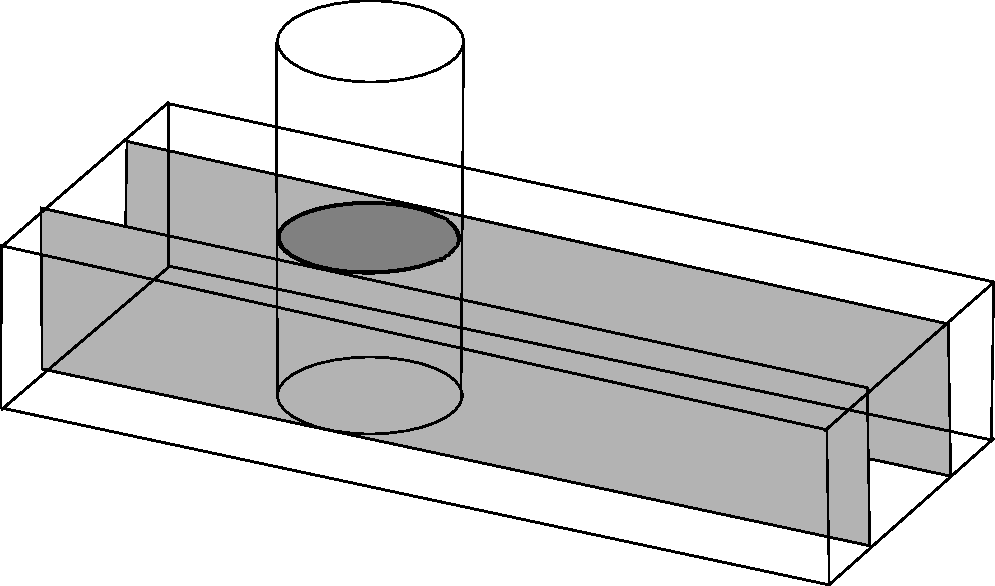
\includegraphics[width=0.6\linewidth]{../Common/images/VolDecomp.pdf}\end{center}
\vspace{-0.8cm}
\begin{center}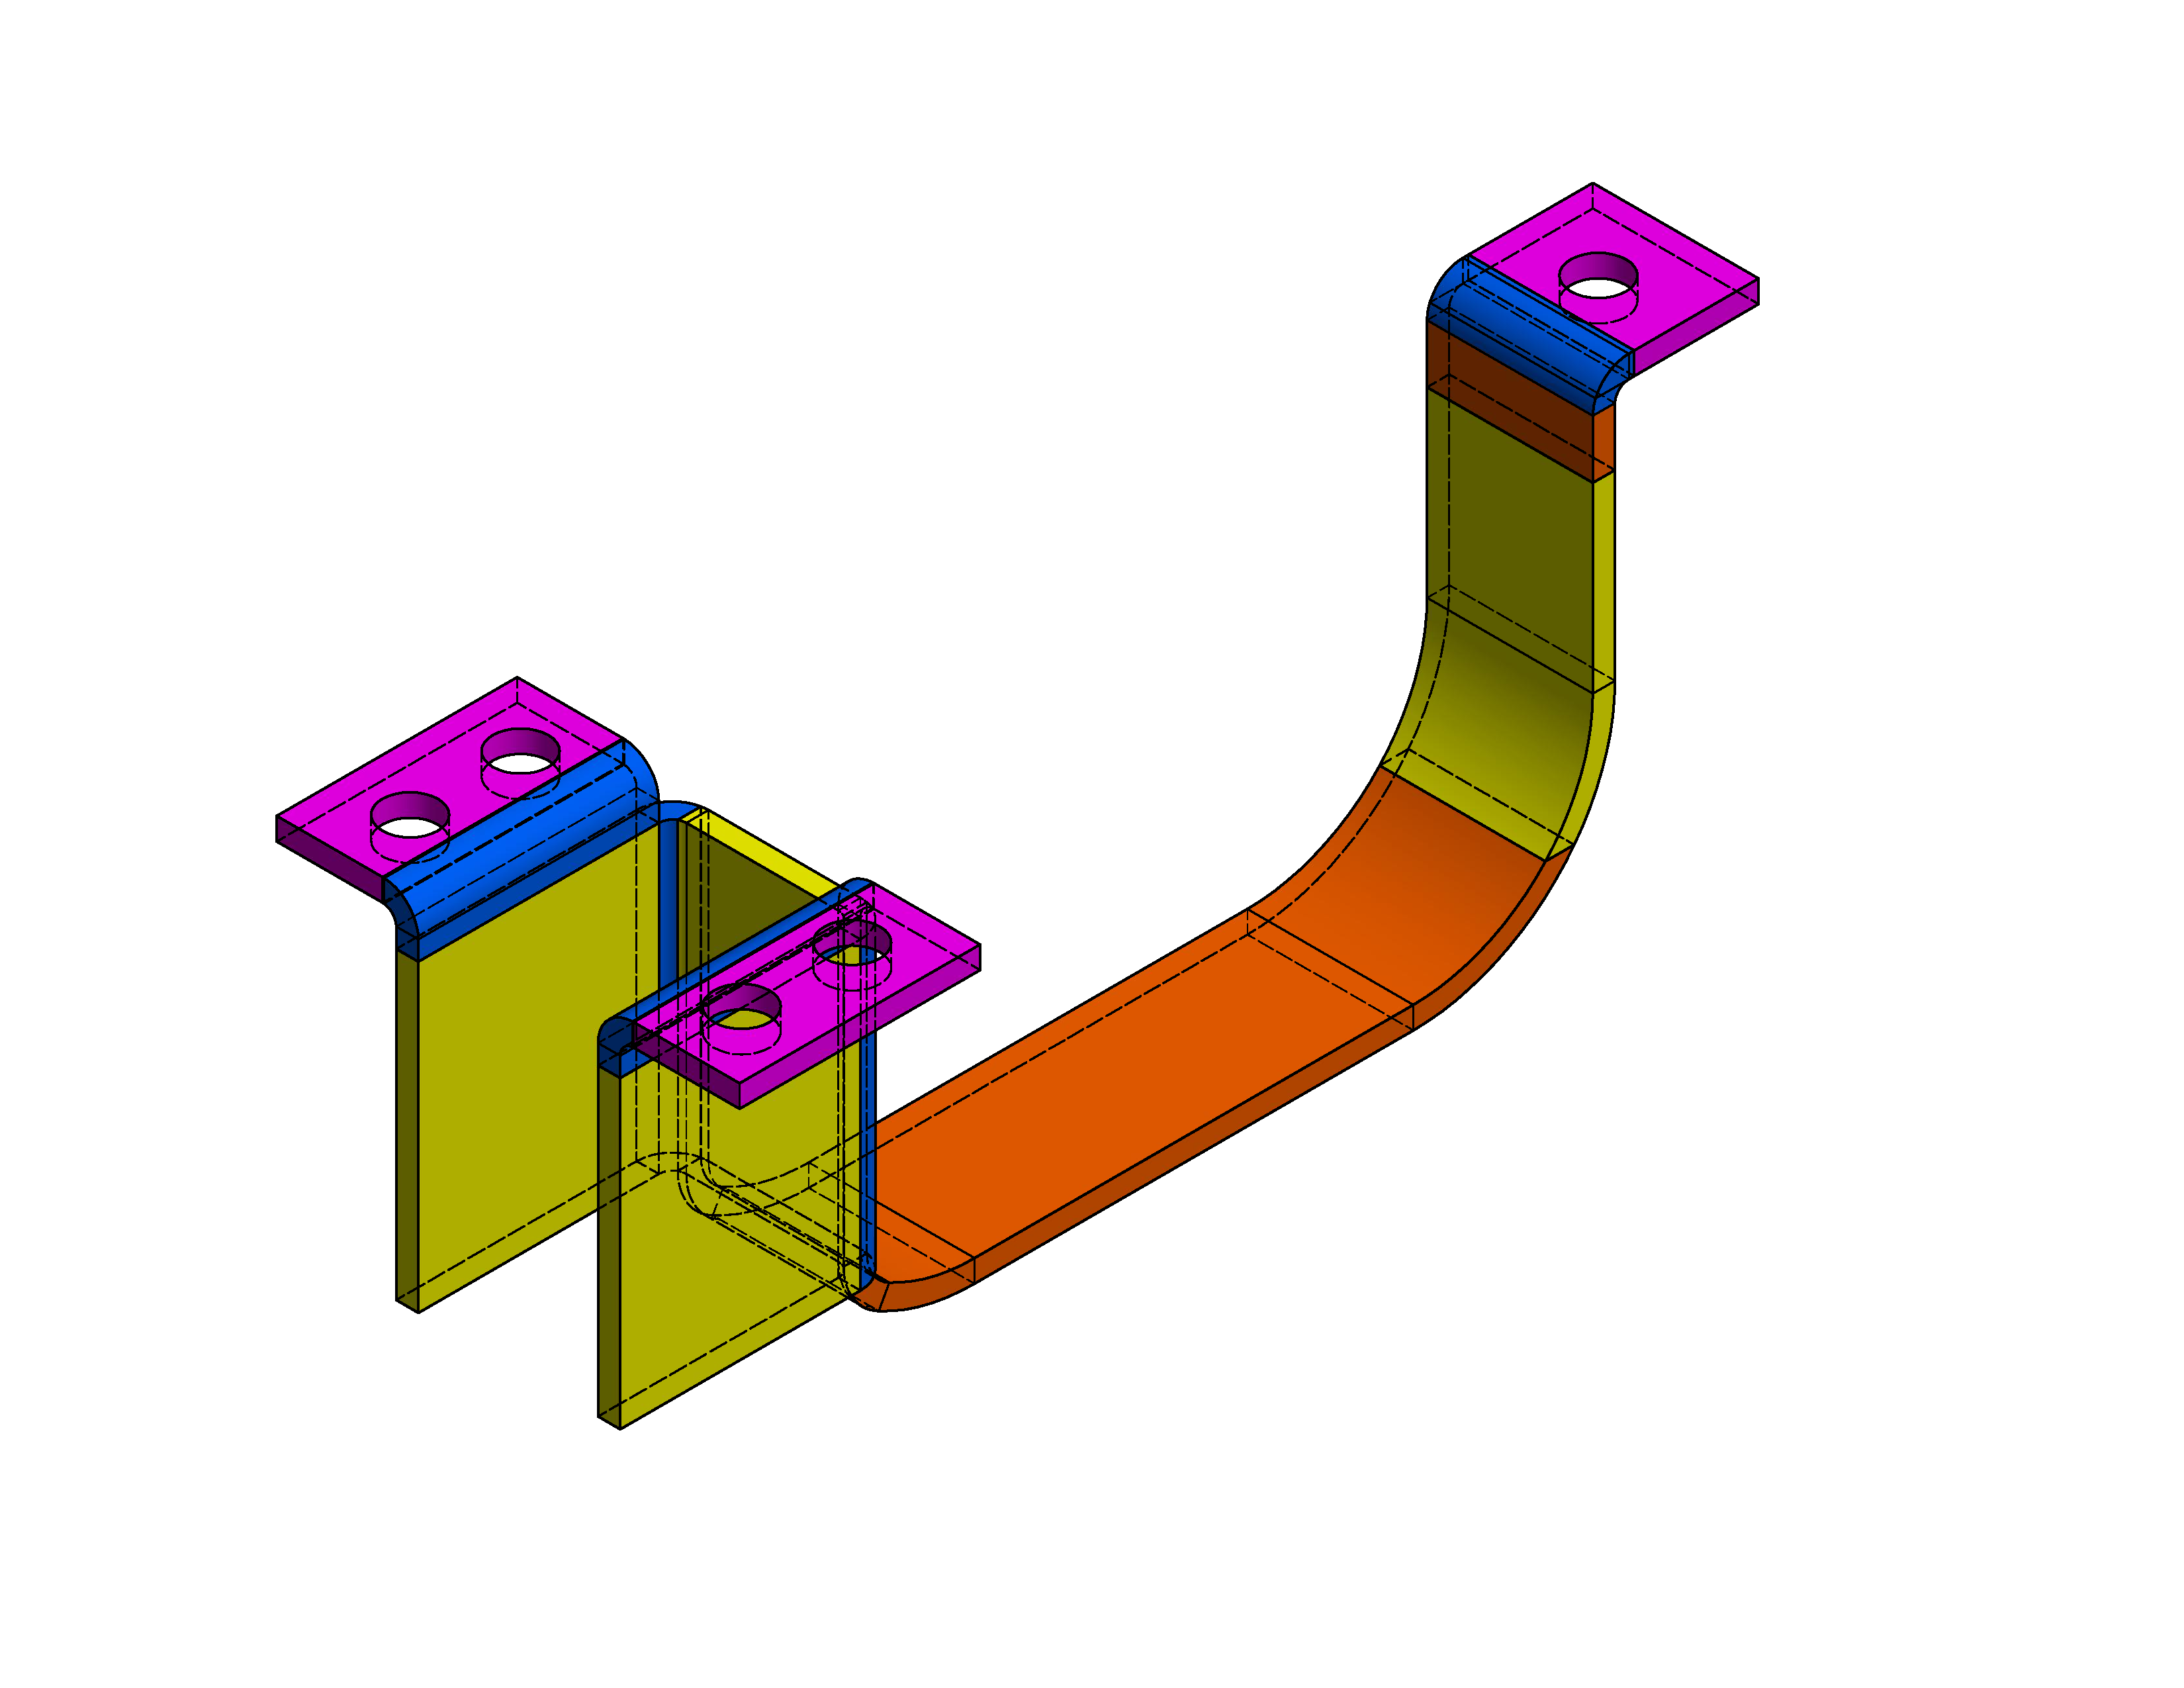
\includegraphics[width=0.6\linewidth]{../Common/images/VolDecomp1.pdf}\end{center}
\vspace{-1.2cm}
The  fundamental unit is called $Cell$, which has dimensionality-$0,1,2,3$ and can have adjacency to its neighbor denoted as $Cell_{dimension,adjacency}$. Actual size and the shape of the cells can vary based on the underlying geometry. Even the actual topological entities may vary due to user-created additional faces/edges by splitting/merging them. But it may be possible to bring such entities to their basic forms, as follows:

\begin{tabular}[h]{@{}p{0.1\linewidth} p{0.1\linewidth} p{0.4\linewidth} p{0.4\linewidth}@{}} 

$Cell_{3,*}$  & 
\adjustbox{valign=t}{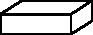
\includegraphics[width=\linewidth]{../Common/images/SimplePlate1.pdf}} &
3D cells (solids), topologically similar to a simple plate &
 $faces=6 \newline edges=12 \newline vertices =8$ \\
 
 $Cell_{2,*}$ &
 \adjustbox{valign=t}{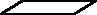
\includegraphics[width=\linewidth]{../Common/images/SimplePlane1.pdf}} &
  2D cells, topologically similar to a planar surface  &
   $faces=1 \newline edges=4 \newline vertices =4$ \\
   
$Cell_{1,*}$ &
 \adjustbox{valign=t}{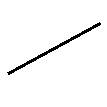
\includegraphics[width=\linewidth]{../Common/images/SimpleLine1.pdf}} &
1D cells, topologically equivalent to a line &
 $edges=1  \newline vertices =2$ \\
 
 $Cell_{3,h}$ &
  \adjustbox{valign=t}{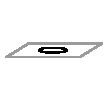
\includegraphics[width=\linewidth]{../Common/images/SimpleHole1.pdf}} &
  Hole is assumed to be cylindrical through-all (true for sheet metal parts) &
   $edges=1  \newline vertices =1$ \\

 \end{tabular}
%	 
%\begin{itemize}
%[noitemsep,topsep=2pt,parsep=2pt,partopsep=2pt]
%	\item $Cell_{3,*}$ : 3D cells, solids, topologically similar to a simple plate 
%	
%	\begin{tabular}[htp]{@{}p{0.2\linewidth} p{0.75\linewidth}@{}} 
%	\adjustbox{valign=t}{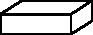
\includegraphics[width=0.9\linewidth]{../Common/images/SimplePlate1.pdf}} &
%	 $faces=6$, $edges=12$, $vertices =8$ \\
%	 \end{tabular}
%	
%	\item $Cell_{2,*}$ : 2D cells (Figure \ref{fig_cellular}b), topologically similar to a planar surface 
%	
%		\begin{tabular}[htp]{@{}p{0.2\linewidth} p{0.75\linewidth}@{}} 
%		\adjustbox{valign=c}{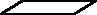
\includegraphics[width=0.9\linewidth]{../Common/images/SimplePlane1.pdf}} &
%		 $faces=1$, $edges=4$, $vertices =4$ \\
%	 	\end{tabular}
%	 	
%	\item $Cell_{1,*}$ : 1D cells, topologically equivalent to a line 
%		\begin{tabular}[htp]{@{}p{0.2\linewidth} p{0.75\linewidth}@{}} 
%		\adjustbox{valign=c}{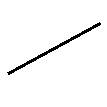
\includegraphics[width=0.55\linewidth]{../Common/images/SimpleLine1.pdf}} &
%		 $edges=1$, $vertices =2$ \\
%	 	\end{tabular}
%
%	\item $Cell_{3,h}$: Hole is assumed to be cylindrical through-all (true for sheet metal parts) 
%			\begin{tabular}[htp]{@{}p{0.2\linewidth} p{0.75\linewidth}@{}} 
%		\adjustbox{valign=c}{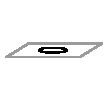
\includegraphics[width=0.9\linewidth]{../Common/images/SimpleHole1.pdf}} &
%		 $edges=1$, $vertices =1$ \\
%	 	\end{tabular}
%\end{itemize}
%
When an original solid is decomposed into distinguishable cells, new interface boundaries are introduced. Newly-created intersecting volumes or touching boundaries are called interface-cells, which can be either 3D (solids) or 2D (faces) respectively. Prefix $s$ is applied if the $Cell$ is from the {\em original solid}, $i$ if it is of a newly-introduced  {\em interface} type, and $m$ for {\em midsurface} cells.

\begin{tabular}[htp]{@{}p{0.48\linewidth} p{0.48\linewidth}@{}} 
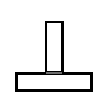
\includegraphics[width=0.6\linewidth]{../Common/images/Interface2d.pdf} 
\label{fig_interfaces} &
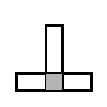
\includegraphics[width=0.6\linewidth]{../Common/images/Interface3d.pdf} \\
2D Interface & 3D Interface\\
\end{tabular}

%\todo[inline]{make two figures in svg 64x64 and change L to T for first figure}


\subsubsection{Steps: Topological Dimension Reduction}
Topological transformation of solid (3D cells) to its corresponding midsurface (2D cells) is as follows:

\begin{itemize}
[noitemsep,topsep=2pt,parsep=2pt,partopsep=2pt]

	\item  $sCell_{3,n}$:	Solid cell with $n$ touching sides transforms into midsurface cell   $mCell_{2,n}$, a surface having $n$ empty edges. Its topological entities are denoted as:
\begin{equation}
f=1,
e=4-n,
v=4-2n
\label{eqn_cellularna}
\end{equation} 

	\item   $sCell_{3,h}$ : Negative solid  cell representing a through hole transforms into midsurface cell  $mCell_{2,h}$, a hole in the surface. Its topological entities are denoted as:
\begin{equation}
e=1, v=1
\label{eqn_cellularah}
\end{equation} 

	\item $iCell_{3,n}$ :	Interface solid cell with $n$ adjacent touching sides transforms into midsurface cell  $mCell_{1,n}$, a radial edge with $n$ leaves. Its topological entities are denoted as:

\begin{equation}
e=1,
v=2
\label{eqn_cellulara}
\end{equation}

	\item  $iCell_{2,2}$ :	Interface face cell touched from both sides  transforms into midsurface cell  $mCell_{1,2}$, a radial edge with 2 leaves. Its topological entities are denoted as:
\begin{equation}
e=1,
v=2
\label{eqn_cellularaf}
\end{equation}


\end{itemize}

%(Eqn   \ref{eqn_cellulara}, \ref{eqn_cellularaf}, \ref{eqn_cellularna}, \ref{eqn_cellularah} )

\subsubsection{Examples}
Table \ref{table_simpleshapes1} lists the various basic shapes and their dimension-reduction-transformations into the corresponding midsurface. 

\todo[inline]{Review A: Correct the number 30.8 in Table 1???}
\todo[inline]{Review C: Minor revision: In section 2.1.2 Examples, adding figures of
decomposed cells from solids would be helpful for readers to
understand the method clearly. Especially, configuration of 
sCells of Y- and rounded L-shape solid is hard to understand 
in a text form. }


\begin{table}[!h]
\caption{Midsurface entities prediction for Simple Shapes}
\begin{tabular}[h]{@{}p{0.1\linewidth} p{0.1\linewidth}  p{0.15\linewidth}  p{0.15\linewidth}  p{0.35\linewidth}@{}} \toprule
{\bf Solid} & {\bf mSurf}  & {\bf sCells} & {\bf mCells}  & {\bf Predicted mSurf Entities} \\ \midrule  

\adjustbox{valign=c}{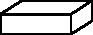
\includegraphics[width=\linewidth]{../Common/images/SimplePlate1.pdf}}  &  
\adjustbox{valign=c}{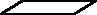
\includegraphics[width=\linewidth]{../Common/images/SimplePlane1.pdf}} &  
$sCell_{3,0}$ & $ mCell_{2,0}$ & 
$ 1f+(4-0)e+(4- 2\times 0)v \newline = 1f+4e+4v$
\\ %\midrule

\adjustbox{valign=c}{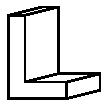
\includegraphics[width=\linewidth]{../Common/images/LPlate1.pdf}}  &  
\adjustbox{valign=c}{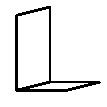
\includegraphics[width=\linewidth]{../Common/images/LPlane1.pdf}} &  

$2 \times sCell_{3,1} \newline + iCell_{3,2}$ & $2 \times mCell_{2,1} \newline + mCell_{1,2}$  & 
$ 2 \times (1f + (4-1)e+(4-2\times 1)v ) \newline + (1e + 2v) \newline = 2f+7e+6v$ 
\\ %\midrule


\adjustbox{valign=c}{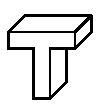
\includegraphics[width=\linewidth]{../Common/images/TPlate1.pdf}}  &  
\adjustbox{valign=c}{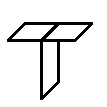
\includegraphics[width=\linewidth]{../Common/images/TPlane1.pdf}} &  

$3 \times sCell_{3,1} + iCell_{3,3}$   &  $3 0.8\times mCell_{2,1}  + mCell_{1,3}$  & 
$3 \times (1f+(4-1)e+ (4-2\times 1)v)  + (1e+2v)  = 3f+10e+8v$ 
\\ %\midrule

\adjustbox{valign=c}{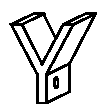
\includegraphics[width=\linewidth]{../Common/images/YwithHole1.pdf}}  &  
\adjustbox{valign=c}{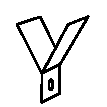
\includegraphics[width=\linewidth]{../Common/images/YwithHolem1.pdf}} &  

$3 \times sCell_{3,1}  + iCell_{3,3}  + sCell_{3,h}$   &  
$3 \times mCell_{2,1}  + mCell_{1,3}  + mCell_{2,h}$  & 
$3 \times (1f+(4-1)e+ (4-2\times 1)v)  + (1e+2v)  + (1e+1v)  = 3f+11e+9v$
\\ %\midrule

\adjustbox{valign=c}{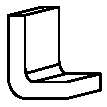
\includegraphics[width=\linewidth]{../Common/images/LwithRound1.pdf}}  &  
\adjustbox{valign=c}{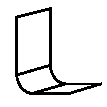
\includegraphics[width=\linewidth]{../Common/images/LwithRoundm1.pdf}} &  

$2 \times sCell_{3,1}  + 2 \times  iCell_{2,2}  + sCell_{3,2}$   &  
$2 \times mCell_{2,1}  + 2 \times mCell_{1,2}  + mCell_{2,2}$  & 
$2 \times (1f+(4-1)e+ (4-2\times 1)v)  + 2 \times (1e+2v)  + (1f+(4-2)e+ (4-2\times 2)v)  = 3f+10e+8v$
\\ 

\bottomrule
\end{tabular}
\label{table_simpleshapes1}
\end{table}

It is evident that the predicted midsurface entities of these simple shapes match with the actual ones, thus the derived formulation works for these simple shapes.  Following is the verification for a relatively-complex practical shape. 

\begin{tabular}[htp]{@{}p{0.48\linewidth} p{0.48\linewidth}@{}} 
{\bf Solid} & {\bf Cellular Classification} \\
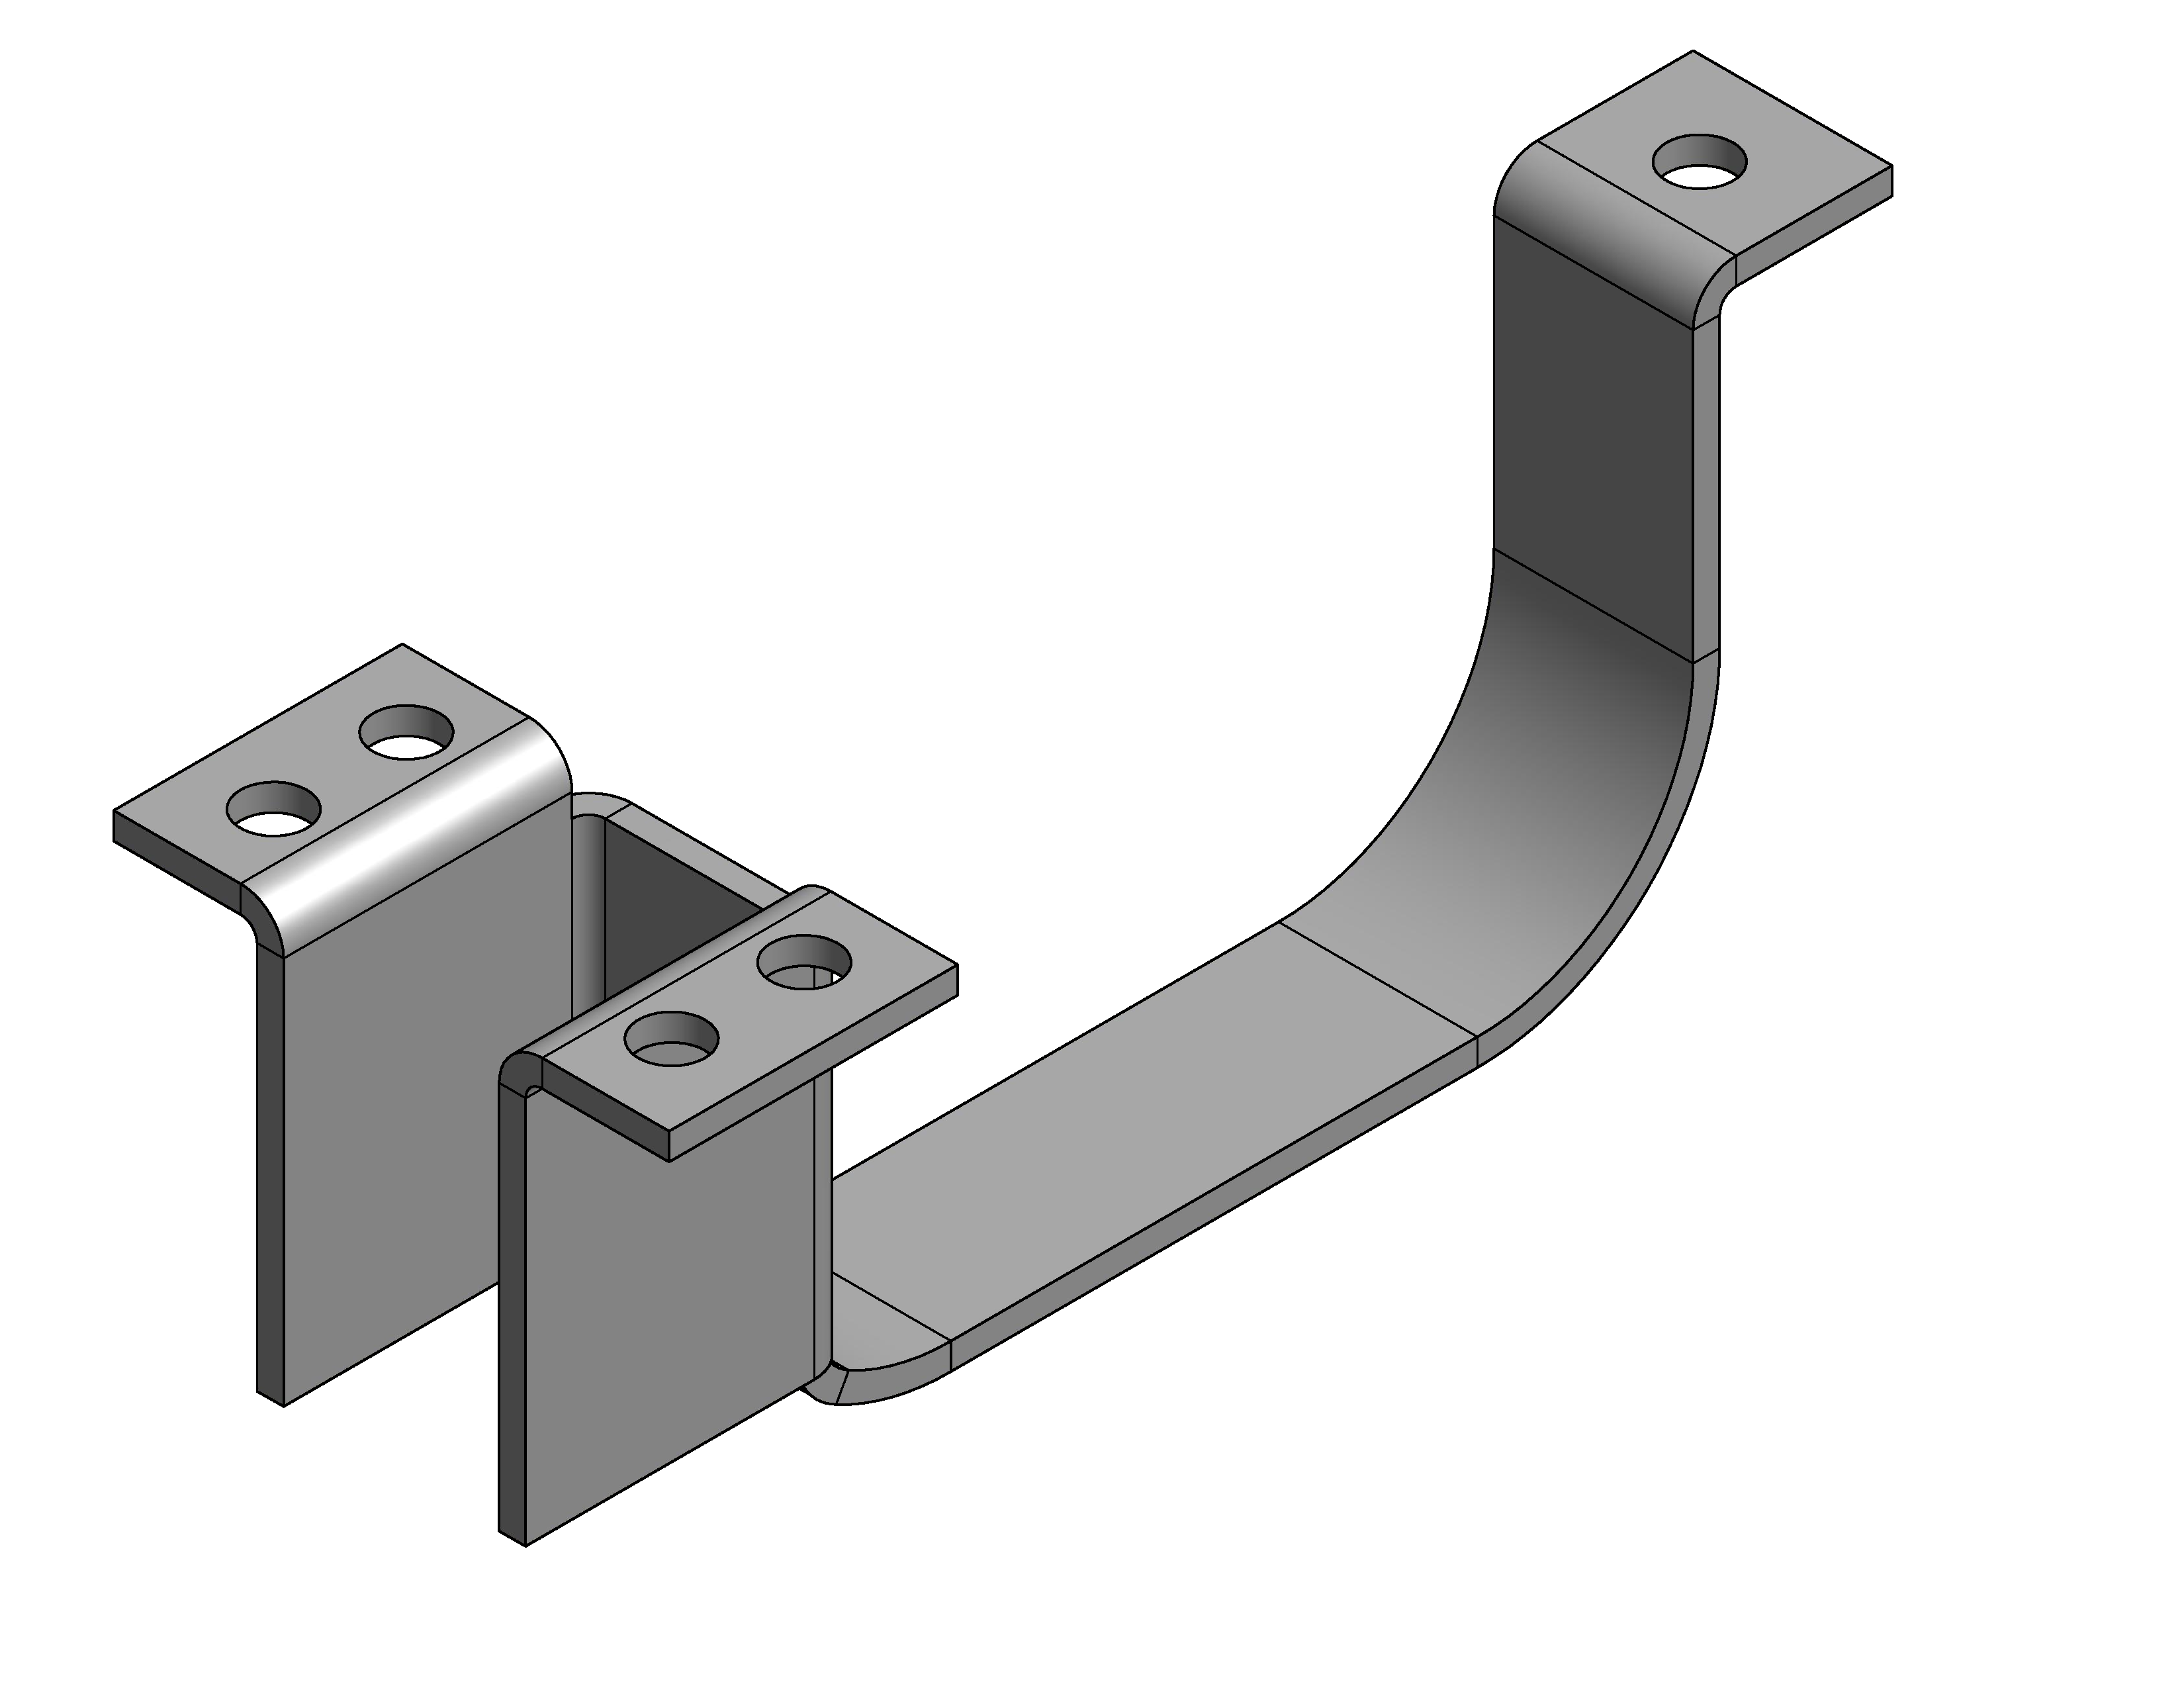
\includegraphics[width=\linewidth]{../Common/images/SimpleBracketshaded.pdf} &
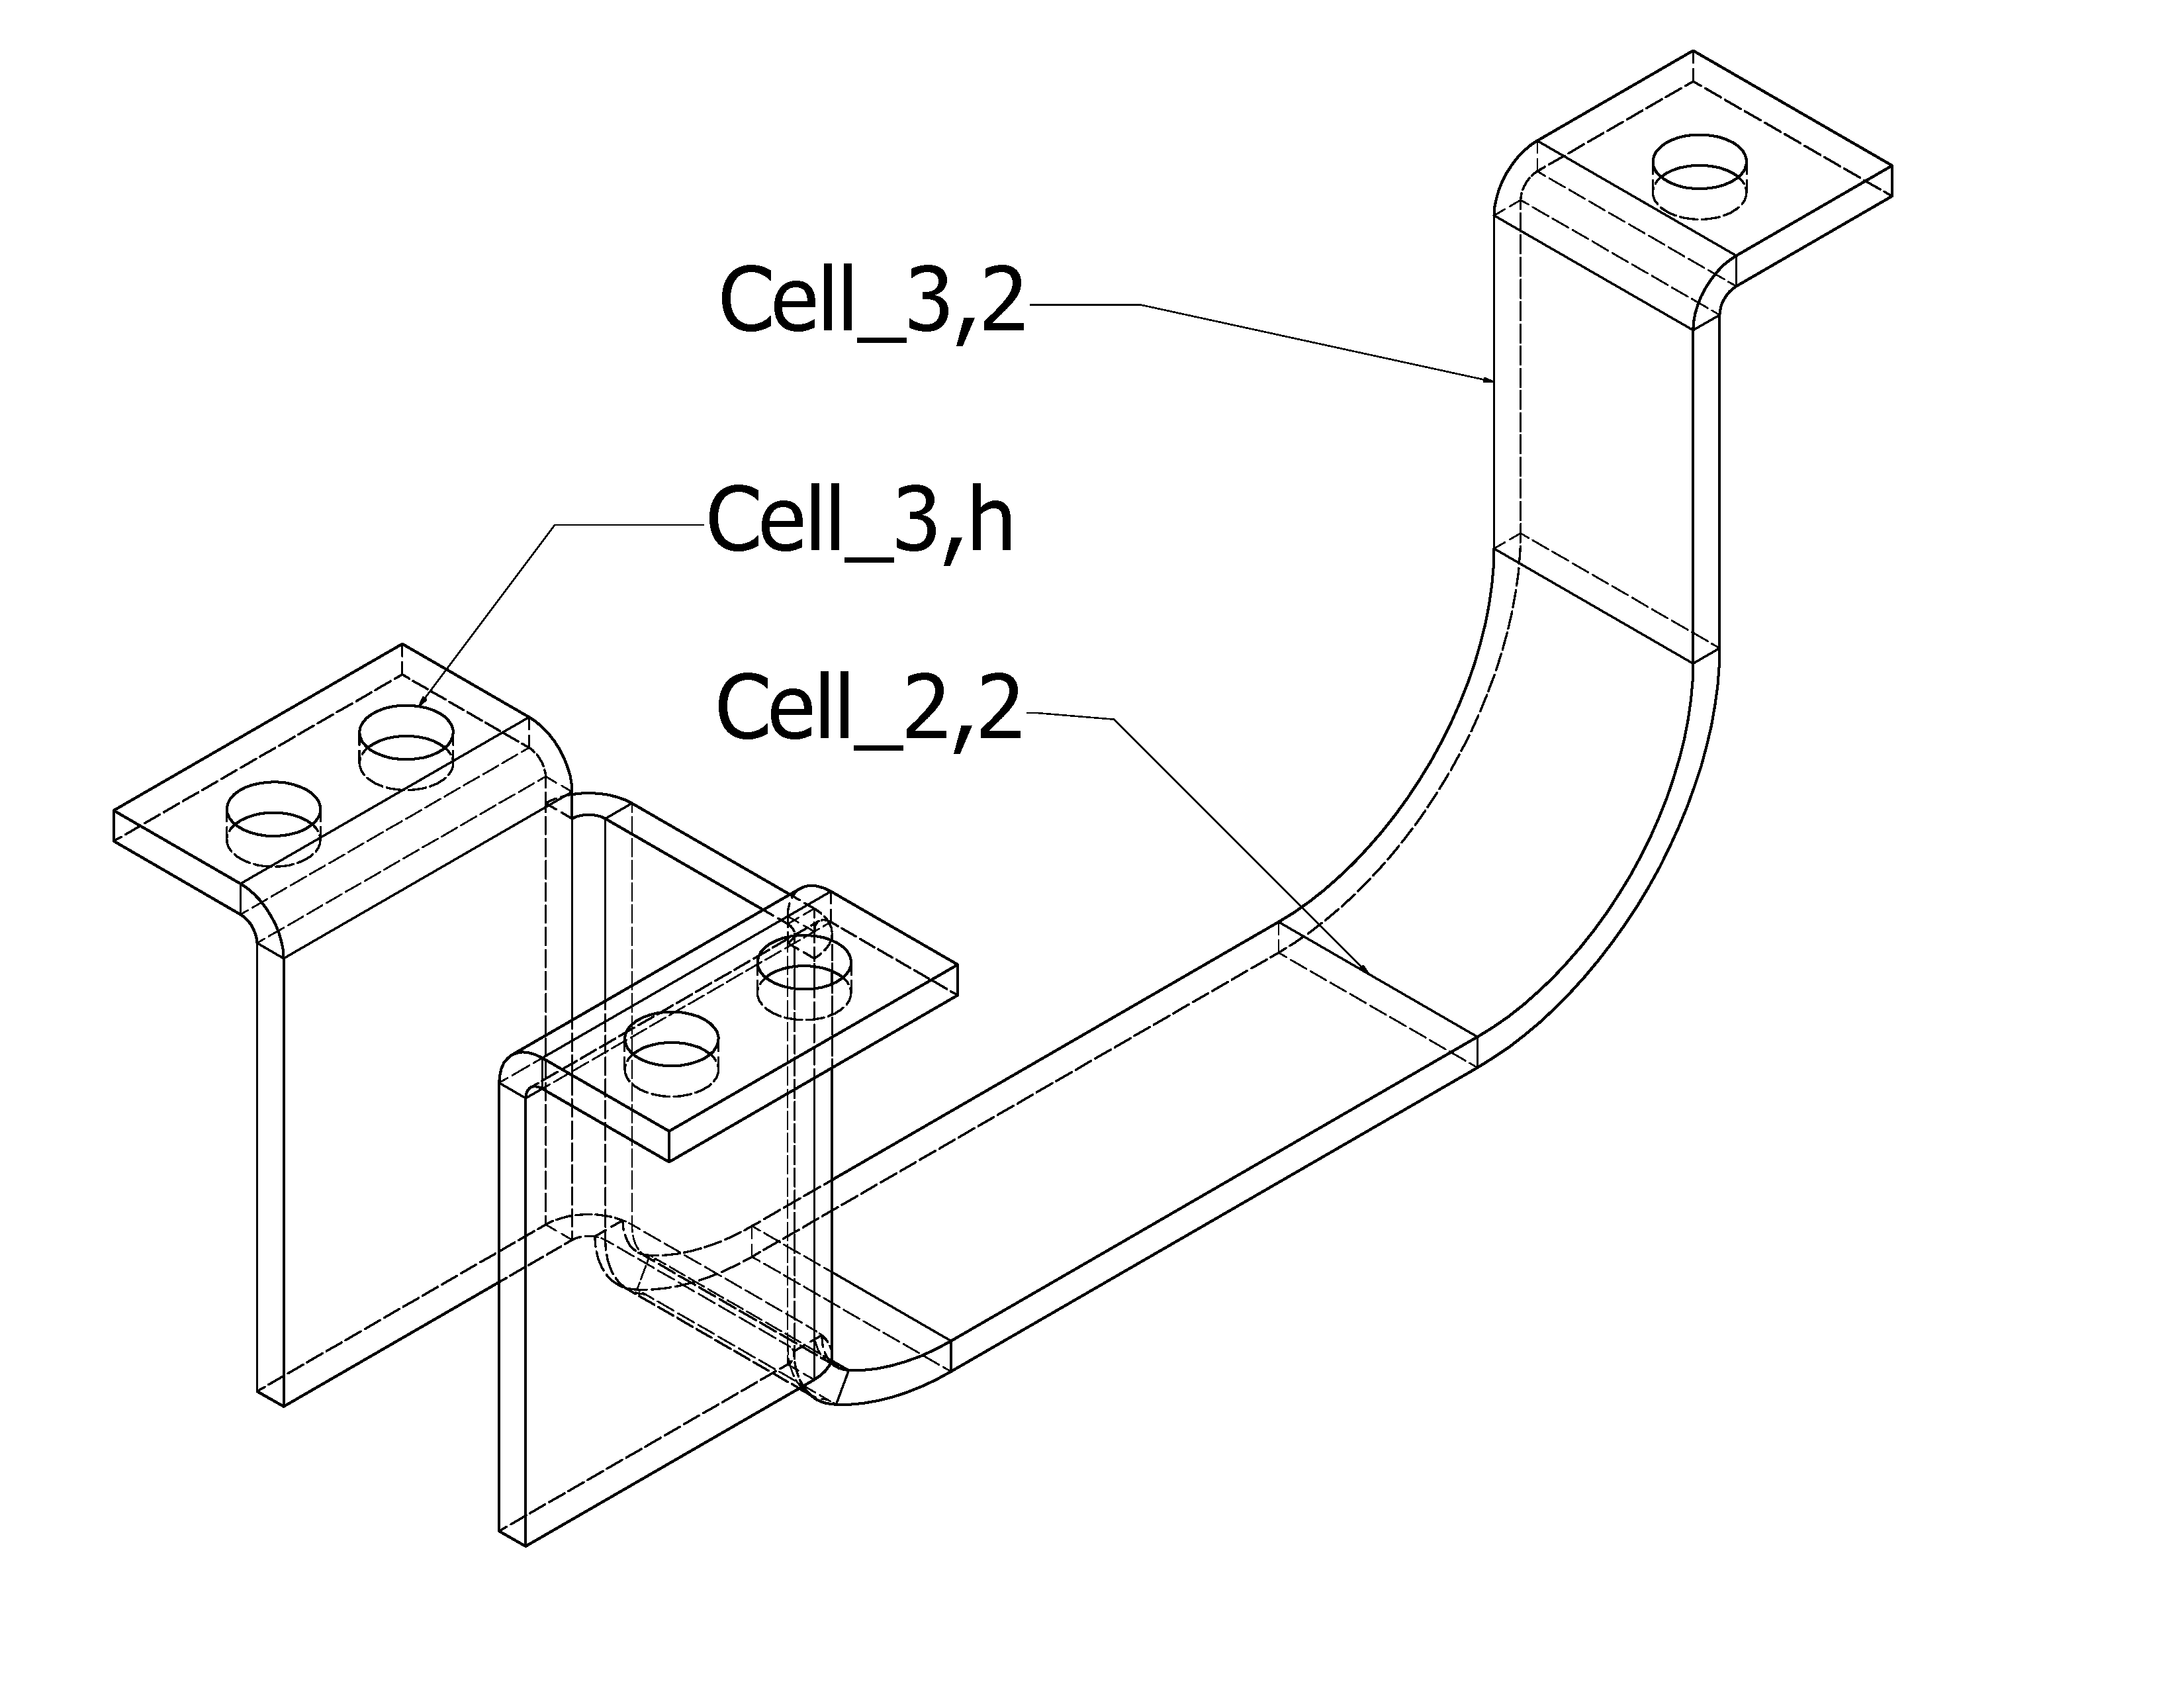
\includegraphics[width=\linewidth]{../Common/images/SimpleBracket.pdf}\\
\end{tabular}

\begin{itemize}
[noitemsep,topsep=2pt,parsep=2pt,partopsep=2pt,leftmargin=*]
	\item \textbf {Solid cells}: \newline  $5 \times sCell_{3,h} + 3 \times sCell_{3,1} + 13 \times sCell_{3,2} + 14 \times iCell_{2,2} $
	\item \textbf {Transformed Midsurface Cells}: \newline $5 \times mCell_{2,h} + 3 \times mCell_{2,1} + 13 \times mCell_{2,2} + 14 \times mCell_{1,2}$
	\item \textbf {Predicated midsurface Entities are}:  \newline $5(1e+1v) + 3 (1f+3e+2v) + 13 (1f+2e+0v) + 14(1e+2v) = 
16f + 54e + 39v$
\end{itemize}
\todo[inline]{Review B:  On page 8 ``Predicated'' should be ``Predicted''}

The derived formulation (Eqn   \ref{eqn_cellulara}, \ref{eqn_cellularaf}, \ref{eqn_cellularna}, \ref{eqn_cellularah} ) predicts correct topological entities for the midsurface. These, when substituted in the non-manifold equation (Eqn \ref{eqn_nonmanifold}) also prove to be valid. With $s=1, r=5, h=5$, the equation matches both sides:
$$ 39 - 54 + (16 -5) = 1 (1-5)$$


\subsection{Midsurface to Sheet Metal Solid Transformation}
In this approach, given a midsurface, topological entities  of its corresponding sheet metal solid are predicted. These predicted entities are verified to check if they validate manifold equation (Eqn \ref{eqn_manifold}).

Topological entities of midsurface contains far richer (classifiable) topological information than its corresponding solid model. For example, midsurface of ``T'' shaped solid, which can be represented as Figure \ref{fig_nonmanifold} has following classified entities:
\todo[inline]{Review B:  On Figure 1 the label ``Radial Edge (v r )'' should be ``Radial Edge (e r )''. Face Uses should have the nomenclature (f u )}

\begin{figure}[htbp]
\begin{center}
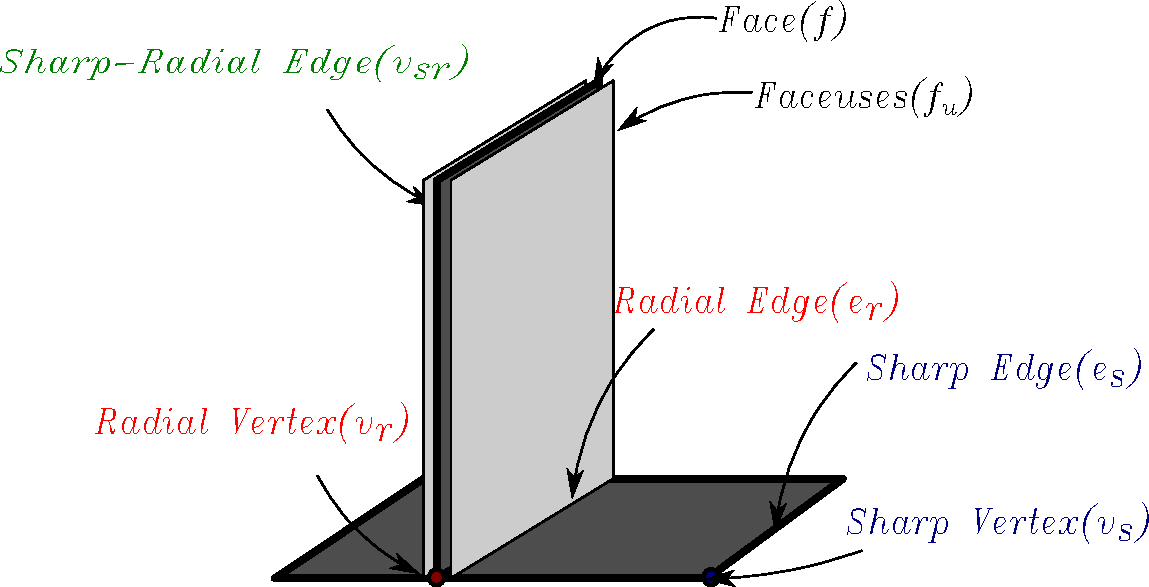
\includegraphics[width=0.6\linewidth]{../Common/images/NonManifoldT1.pdf} 
\end{center}
\caption{Classification of topological entities of the midsurface}
\label{fig_nonmanifold}
\end{figure}

	\begin{itemize} 
	[noitemsep,topsep=2pt,parsep=2pt,partopsep=2pt,label={}]\label{list_topos}
	\item Faces ($f$): Bound by two face-uses $f_u$.
	
	\item Sharp Vertex ($v_s$): Connected to two edges of the same face
	\item Sharp Edge ($e_s$): Connected to two sharp vertices

	\item Radial Vertex ($v_{r}$): Connected edges of different faces
	\item Degree ($n_{r}$) at the radial edge is the number of faces attached to it 
	\item Cross Radial Edge ($e_{r}$): Connected between two radial vertices and connects two different faces
	\item Side-Radial  Edge ($e_{rr}$): Connected between two radial vertices and is of same face
	\item Sharp-Radial Edge ($e_{sr}$): Between sharp and radial vertex
	\item Internal Edge ($e_i$): Part of the inner loop
	\item Internal Vertex ($v_i$):Connected to the internal edge
	\item Internal Loop ($r_i$) : Characterized by internal edges and vertices
	\end{itemize}

\subsubsection{Steps: Topological Dimension Addition}
Sheet Metal part can be imagined to be thickened midsurface \cite{SHLee2001}. The topological entities of the generated solid are calculated as per following steps: %via relations in the Table \ref{table_TopoVal}.

%\begin{itemize}
%[noitemsep,topsep=2pt,parsep=2pt,partopsep=2pt]


%\begin{center} 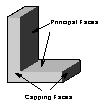
\includegraphics[width=0.5\linewidth]{../Common/images/PrincipalCappingL1.pdf}
%\end{center}


\begin{tabular}[htp]{@{}p{0.6\linewidth} p{0.3\linewidth}@{}} 

	\begin{itemize}
	[noitemsep,topsep=2pt,parsep=2pt,partopsep=2pt,leftmargin=*]
	\item Face-uses become principal faces. 
 
\item Sharp vertices create capping edges.

%\item Face-uses around a radial edge remain as connected in the solid as well. 
%Face-uses of same face will get connected via thickness faces
\item Apart from edge-use loop corresponding to face-use, a new loop is proposed for side-capping faces. The loop is formed between two sharp vertices ($v_s$) using  more than one sharp  ($e_{sr}$) or side radial ($e_{rr}$) edges but not using the cross radial edge ($e_r$). Such independent paths creating individual side faces are called $l_p$.

	\item Loop between two sharp vertices. This gives rise to a singular capping face  (Fig. a).
	\item Loop between three branched sharp vertices. This gives rise to a combined capping face (Fig. b).
	\item Loop between two sharp vertices with multiple radial vertices in between them. This gives rise to a combined capping face (Fig. c).
	\end{itemize}
	&
\adjustbox{valign=t}{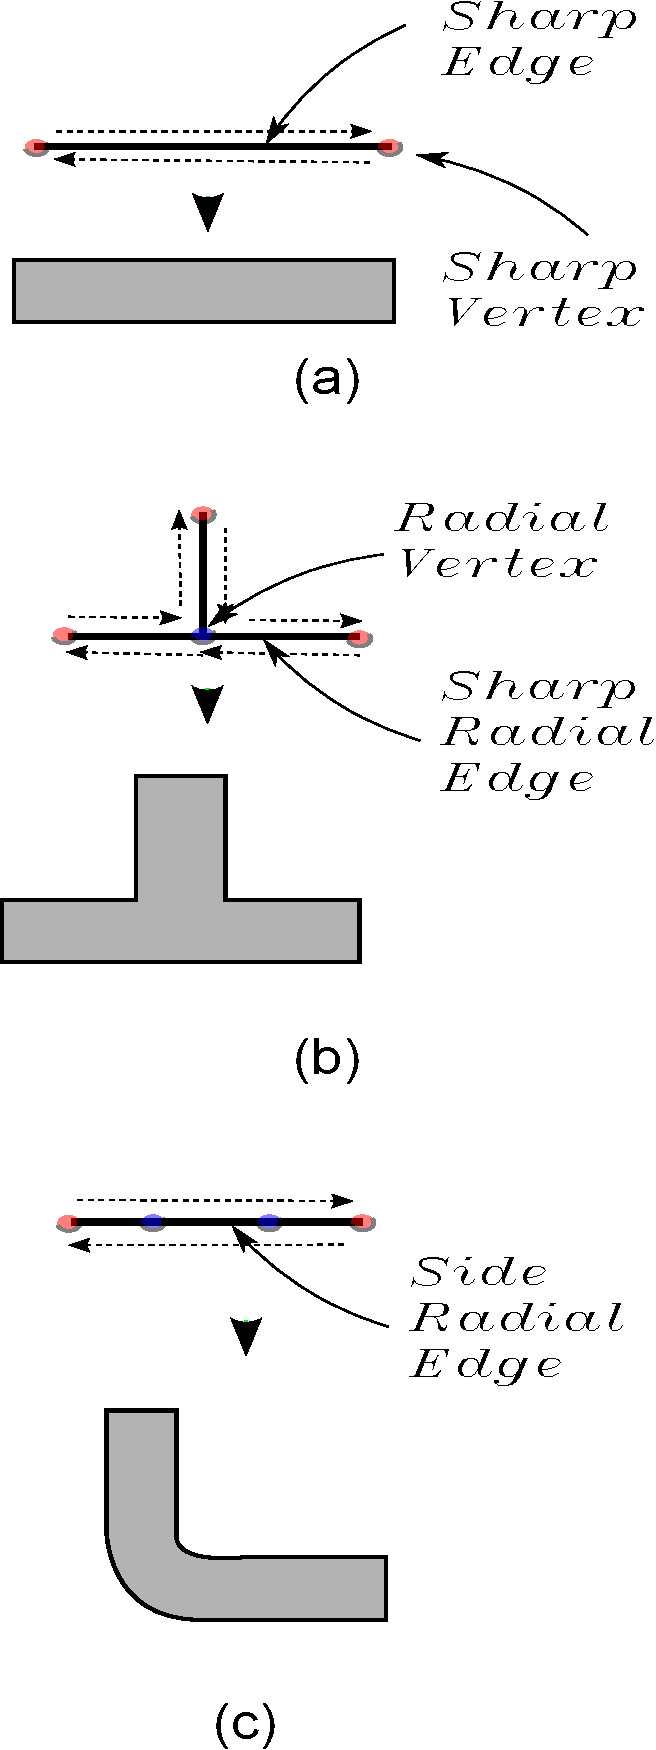
\includegraphics[height=2\linewidth]{../Common/images/NonManifoldLoopsToFaces1.pdf}} \\
\end{tabular}



	

%\item Radial vertices or edges won't create any new topological entity
%\end{itemize}


Topological entities in the thickened solid are predicted as follows:% (Summary in Table \ref{table_TopoVal}):
\begin{itemize}
[noitemsep,topsep=2pt,parsep=2pt,partopsep=2pt,label=\textbullet]
\item Manifold-Vertices  ($v_m$) = Double the sharp and internal vertices (one up  and  one below) + vertices for junctions of which are denoted by the summation of  number of radial vertices times their corresponding degrees
\begin{equation}
v_m = 2 (v_s + v_i) + \sum n_{r} v_{r} \label{eqn_vm}
\end{equation}
\item Manifold-Edges ($e_m$)= two times sharp, sharp-radial and internal edges (offset up and down) + degree times radial edges for offsets at junctions + sharp vertices for vertical-capping edges + internal vertices for vertical seam edges
\begin{equation}
e_m = 2 (e_s + e_{sr} + + e_{rr} + e_i) + \sum n_r e_r  + v_s + v_i\label{eqn_em}
\end{equation}
\item Manifold-Faces ($f_m$) = Double the faces (offset up and down) + sharp edges for capping faces + paths to have one combined face + internal edges for capping internal faces
\begin{equation}
f_m = 2f + e_s + l_p + e_i \label{eqn_fm}
\end{equation}
\item Manifold-Shells ($s_m$) = Remains the same
\item Manifold-Rings ($r_m$) = Two times the internal rings
\begin{equation}
r_m = 2r_i\label{eqn_rm}
\end{equation}
\item Manifold-Genus ($h_m$) = Internal ring as it becomes a hole
\begin{equation}
h_m = r_i\label{eqn_hm}
\end{equation}

\end{itemize}
%
%\begin{table}
%\caption{Solid by thickening midsurface Entities}
%\begin{tabular}[]{@{} p{0.25\linewidth}  p{0.25\linewidth}  p{0.4\linewidth}@{}} \toprule
%{\bf Solid } & {\bf Midsurface }  & {\bf Explanation} \\
%\midrule
%%------------------------------------------------------------------------------------------------------------------------------------
%Faces ($f_m$) &
%$2f+e_s+e_{sr}/n_{r} +e_i $ &
%Double faces to make Main faces + Thickness faces + Common faces for Loop with Radial in it + inner hole face \\
%%------------------------------------------------------------------------------------------------------------------------------------
%Edges ($e_m$) &
%$2(e_s+e_{sr}+e_i )+n_{r} e_{r}+v_s+v_i  $ &
%Double (sharp + sharp-radial + internal) to represented offseted edges + $n$ edges radially offseted from $e_r$ + thickness edges one per sharp vertex + seam edge + internals\\
%%------------------------------------------------------------------------------------------------------------------------------------
%Vertices ($v_m$) &
%$2v_s+n_{r} v_r+2v_i$ &
%Double offseted vertices + $n$ times offsetting at each $v_r$+ double the offseted seam vertices\\
%%------------------------------------------------------------------------------------------------------------------------------------
%Shell ($s_m$) &
%$s$ &
%Same\\
%%------------------------------------------------------------------------------------------------------------------------------------
%Rings ($r_m$) &
%$2r_i $& 
%Double for offsetting. Assuming sheet metal generated only through hole and not the blind hole.\\
%%------------------------------------------------------------------------------------------------------------------------------------
%Genus  ($h_m$) &
%$r_i $&
%Through holes == genus\\
%%------------------------------------------------------------------------------------------------------------------------------------
%
%\bottomrule
%\end{tabular}
%\label{table_TopoVal}
%\end{table}

%\subsubsection{Sheet Metal Midsurface Characteristic}
%Quantifying paths ($l_p$) is not possible $a priori$ as it depends on the actual connections and configurations of the sub-shapes. As paths are typically vary via multiple Side-Radial edges ($e_{rr}$), as simplified case can be assumed for no such edges. So configurations where only Sharp-Radial edges ($e_{sr}$) are present, $l_p$ gives rise to $\frac{e_{sr}}{n_r}$ faces.
%The predicted manifold entities (Equations \ref{eqn_vm}, \ref{eqn_em}, \ref{eqn_fm}, \ref{eqn_rm}, \ref{eqn_hm}) if honor the manifold eqution (Eqn. \ref{eqn_manifold}), then the midsurface can be treated as a valid representation of the sheet metal part. 
%
%%\vspace{-3mm}
%\begin{equation}
%v_m-e_m+f_m=2(s_m-h_m )+r_m
%\label{eqn_predictedmanifold}
%\end{equation}
%
%Substitute for each manifold entities to get:
%%\begin{itemize}
%%[noitemsep,topsep=2pt,parsep=2pt,partopsep=2pt,label={}]
%%\item $v_m = 2v_s+n_{r} v_r+2v_i $
%%\item $e_m = 2(e_s+e_{sr}+e_i )+n_{r} e_{r}+v_s+v_i $
%%\item $f_m = 2f+e_s+e_{sr}/n_{r} +e_i $
%%\item $r_m = 2r_i, h_m = r_i$ ({\em genus} is half the loops)
%%\end{itemize}
%
%%\vspace{-5mm}
%\begin{multline}
%[2 (v_s + v_i) +n_{r} v_r ]\\
%-[2(e_s+e_{sr}+e_i )+n_{r} e_{r}+v_s+v_i ]\\
%+[2f+e_s+e_{sr}/n_{r} +e_i ]\\
%=2(s-r_i )+2r_i
%\label{eqn_midsurf}
%\end{multline}
%
%Midsurface entities should also honor the non-manifold equation (\ref{eqn_nonmanifold}):
%%\vspace{-2mm}
%\begin{equation}
%v-e+f=1(s-h)+r
%\label{eqn_predictednonmanifold}
%\end{equation}
%
%Expanding it with classified entities as below:
%% \vspace{-3mm}
%\begin{align}
%[v_s+v_r+v_i]-[e_s+e_r+e_{sr}+e_i ]+[f]\\=1(s-r_i )+r_i
%\label{eqn_nonmanifoldexpanded}
%\end{align}
%
%(Equation \ref{eqn_midsurf}) - 2 $\times$ (Equation  \ref{eqn_nonmanifoldexpanded}) gives
%%\vspace{-3mm}
%\begin{align}
%v_s+(2-n_{r} ) v_{r}+v_i \\= e_s+e_i+(2-n_{r}) e_{r}+e_{sr}/n_{r}\\=\chi_{smm}
%\label{eqn_nonmanifolddiff}
%\end{align}
%
%This is the new sheet metal midsurface Characteristic  $\chi_{smm}$. It is just in terms of $edges$ and $vertices$. One has to check only this equation on midsurface entities and then it is sure that the corresponding solid manifold (computed by thickening) will be valid as well.
%
%

%\subsubsection{Procedure to validate midsurface using  $\chi_{smm}$}
\subsubsection{Procedure to Validate Midsurface}
\begin{enumerate}
\item Count topological entities of the midsurface as per the classification suggested : \\$f, e_s , e_{sr} , e_{rr}, e_r , e_i, v_s , v_r , v_i, s , h , r$ (more details in Section \ref{list_topos}) .
\item Predict topological entities of the corresponding thin-walled solid using equations ( \ref{eqn_vm}, \ref{eqn_em}, \ref{eqn_fm}, \ref{eqn_rm}, \ref{eqn_hm}).
	\begin{enumerate}
%		\item Predicted solid-faces: $f_m \\= 2f+e_s+e_{sr}/n_{r} +e_i $
		\item Predicted solid-faces: $f_m \newline = 2f+e_s+ l_p +e_i $
		\item Predicted solid-edges: $e_m \newline = 2(e_s+e_{sr}+e_{rr}+e_i )+ \sum n_{r} e_{r}+v_s+v_i $
		\item Predicted solid-vertices: $v_m \newline= 2v_s+ \sum n_{r} v_r+2v_i$
		\item Predicted solid-shells-holes: \newline$s_m =s = 1, h_m = r_i  = 0, r_m = 2r_i = 0$
		\item Non-manifold equation of the left side  $\chi_{nml} \newline= v-e+f $
		\item Non-manifold equation of the  right side  $\chi_{nmr} \newline=s-h+r$
		\item Manifold equation of the  left side  $\chi_{ml} \newline= v_m-e_m+f_m $
		\item Manifold equation of the  right side  $\chi_{mr}\newline=2(s_m-h_m )+r_m$
%		\item Sheet metal midsurface characteristic $\chi_{smm} \\=
%		e_s+e_i+(2-n_{r} ) e_{r}+e_{sr}/n_{r} =v_s+(2-n_{r} ) v_{r}+v_i$
	\end{enumerate}
\item Verify that the topological entities of the midsurface satisfy the non-manifold equation (Equation \ref{eqn_nonmanifold}), by deducing that the left ($\chi_{nml}$) and right  ($\chi_{nmr}$) hand side of the equation matches.
\item Verify that the predicted topological entities of the  thin-walled solid satisfy the manifold equation (Equation \ref{eqn_manifold}), by deducing that the left ($\chi_{ml}$) and right  ($\chi_{mr}$) hand side of the equation match; thus proving that the transformation equations are valid. 
%Same validity can be shown using just the $\chi_{smm}$ characteristic, as below.
%\item Verify that  $\chi_{smm}$ characteristic equation (Equation \ref{eqn_nonmanifolddiff}) matches. 
\end{enumerate}



\subsubsection{Examples}
Table \ref{table_simpleshapes2} displays the validation of midsurface using proposed dimension-addition-transformation equations.

%\begin{enumerate}
%[noitemsep,topsep=2pt,parsep=2pt,partopsep=2pt,leftmargin=*]
%\item Simple Plate %(Table \ref{table_TopoValPlate})
%
%%\vspace{3mm}
%\begin{center}
%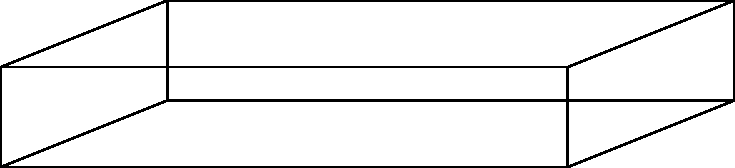
\includegraphics[width=0.35\linewidth]{../Common/images/SimplePlate.pdf} 
%\end{center}
%%\vspace{3mm}
%
%\begin{enumerate}
%%[noitemsep,topsep=2pt,parsep=2pt,partopsep=2pt,label=\textbullet,leftmargin=*]
%\item Midsurface entities: \\$f = 1, e_s = 4, e_{sr} = 0, e_r = 0, e_i=0,$\\$v_s = 4,v_r =0, v_i= 0, s=1,h=0,r=1$
%\item Predicted solid-faces: \\$f_m = 2f+e_s+e_{sr}/n_{r} +e_i $\\$= 2+4+0+0 = 6$
%\item Predicted solid-edges: \\ $e_m = 2(e_s+e_{sr}+e_i )+n_{r} e_{r}+v_s+v_i $\\$= 2(4+0+0)+0+4+0 = 12$
%\item Predicted solid-vertices: \\$v_m = 2v_s+n_{r} v_r+2v_i$\\$=2\times4 + 0 + 0=8$
%\item Predicted solid-shells-holes: \\$s_m =s = 1, h_m = r_i  = 0, r_m = 2r_i = 0$
%\item Non-manifold equation left side  $\chi_{nm-left} $\\$= v-e+f $\\$= 4-4+1 = 1$
%\item Non-manifold equation right side  $\chi_{nm-right}$\\$=s-h+r$\\$=1-0+0 = 1$
%\item Manifold equation left side  $\chi_{m-left} $\\$= v_m-e_m+f_m $\\$=8-12+6= 2$
%\item Manifold equation right side  $\chi_{m-right}$\\$=2(s_m-h_m )+r_m$\\$= 2(1-0)+0 = 2$
%\item Sheet metal midsurface characteristic $\chi_{smm}$\\$=
%e_s+e_i+(2-n_{r} ) e_{r}+e_{sr}/n_{r} $\\$=v_s+(2-n_{r} ) v_{r}+v_i$\\$ 4+0+0+0=4+0+0= 4$
%\item \textbf{Result}: \textcolor{green}{Matches}
%\end{enumerate}
%\item Y with hole on one leg% (Table \ref{table_TopoValY})
%
%%\vspace{3mm}
%\begin{center}
%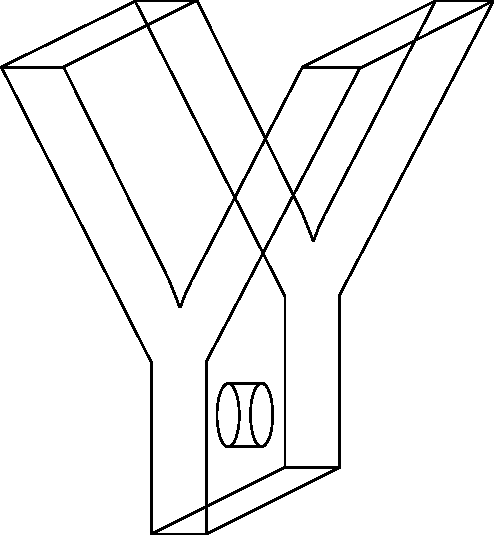
\includegraphics[width=0.3\linewidth]{../Common/images/YwithHole.pdf} 
%\end{center}
%%\vspace{3mm}
%
%\begin{enumerate}
%%[noitemsep,topsep=2pt,parsep=2pt,partopsep=2pt,label=\textbullet,leftmargin=*]
%\item Midsurface entities: \\ $f = 3, e_s = 3, e_{sr} = 6, e_r = 1, e_i=1,v_s = 6,v_r =2, v_i= 1, s=1,h=0,r=1$
%\item Predicted solid-faces: \\ $f_m = 2f+e_s+e_{sr}/n_{r} +e_i  $\\$= 6+3+2+1=12$
%\item Predicted solid-edges: \\$e_m = 2(e_s+e_{sr}+e_i )+n_{r} e_{r}+v_s+v_i $\\$= 2(3+6+1)+3+6+1 =30$
%\item Predicted solid-vertices:  $v_m = 2v_s+n_{r} v_r+2v_i $\\$=2\times6+ 6 + 2=20$
%\item Predicted solid-shells-holes: $s_m =s = 1,h_m = r_i  = 1, r_m = 2r_i = 2$
%\item Non-manifold equation left side  $\chi_{nm-left}$\\$= v-e+f $\\$= 9-11+3=1$
%\item Non-manifold equation right side  $\chi_{nm-right}$\\$=s-h+r$\\$=1-1+1 = 1$
%\item Manifold equation left side  $\chi_{m-left}$\\$= v_m-e_m+f_m$\\$=20-30+12 = 2$
%\item Manifold equation right side  $\chi_{m-right} $\\$=2(s_m-h_m )+r_m$\\$= 2(1-1)+2 = 2$
%\item Sheet metal midsurface characteristic $\chi_{smm}$ \\$=
%e_s+e_i+(2-n_{r} ) e_{r}+e_{sr}/n_{r} $\\$=v_s+(2-n_{r} ) v_{r}+v_i$\\$ 3+1+(2-3)+2=6+(2-3)2+1=5$
%\item \textbf{Result}: \textcolor{green}{Matches}
%\end{enumerate}

\begin{table}
\caption{Sheet Metal Characteristics usage, Simple examples}
\begin{tabular}[t]{@{} p{0.08\linewidth}  
p{0.02\linewidth}  p{0.02\linewidth}  p{0.02\linewidth}   p{0.02\linewidth}  p{0.02\linewidth}  p{0.02\linewidth}     p{0.02\linewidth}  p{0.02\linewidth}  p{0.02\linewidth} p{0.02\linewidth}  p{0.02\linewidth}  p{0.02\linewidth}  p{0.02\linewidth}   p{0.02\linewidth} @{}} \toprule
{\bf mSurf} & 
{\bf $f$}  		& {\bf $l_p$ } 	& {\bf $e_s$ }  	& {\bf $e_{sr}$} & {\bf $e_r$}  & 
{\bf $e_{rr}$} 	& {\bf $e_i$ } 	& {\bf $v_s$ } 	& {\bf $v_r$}  	&  {\bf $v_i$}  & 
{\bf $f_{m}$} 	& {\bf $e_m$ } 	& {\bf $v_m$ } 	& {\bf $\chi_{m*}$ } \\ \midrule 

\adjustbox{valign=c}{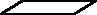
\includegraphics[width=\linewidth]{../Common/images/SimplePlane1.pdf}}  &  
1 & 0 & 4 & 0 & 0 & 0 & 0  & 4 & 0 & 0 & 6 & 12 & 8 & 2 \\ 

\adjustbox{valign=t}{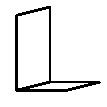
\includegraphics[width=\linewidth]{../Common/images/LPlane1.pdf}}  &  
2 & 2 & 2 & 4 & 1 & 0 & 0  & 4 & 2 & 0 & 8 & 18 & 12 & 2 \\ 


\adjustbox{valign=t}{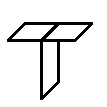
\includegraphics[width=\linewidth]{../Common/images/TPlane1.pdf}}  &  
3 & 2 & 3 & 6 & 1 & 0 & 0  & 6 & 2 & 0 & 11 & 27 & 18 & 2 \\ 

\adjustbox{valign=c}{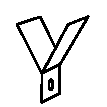
\includegraphics[width=\linewidth]{../Common/images/YwithHolem1.pdf}}  &  
3 & 2 & 3 & 6 & 1 & 0 & 1  & 6 & 2 & 1 & 12  &  30  & 20  & 2 \\ 

\adjustbox{valign=c}{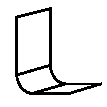
\includegraphics[width=\linewidth]{../Common/images/LwithRoundm1.pdf}}  &  
3 & 2 & 2 & 4 & 2 & 2 & 0  & 4 & 4 & 0 & 10  & 24  & 16  & 2 \\  
\bottomrule
\end{tabular}
\label{table_simpleshapes2}
\end{table}

It is evident that the derived formulation works for simple shapes. 

Following is the verification for a relatively-complex practical shape.

\begin{tabular}[htp]{@{}p{0.48\linewidth} p{0.48\linewidth}@{}} 
{\bf Midsurface} & {\bf Edge Classification} \\
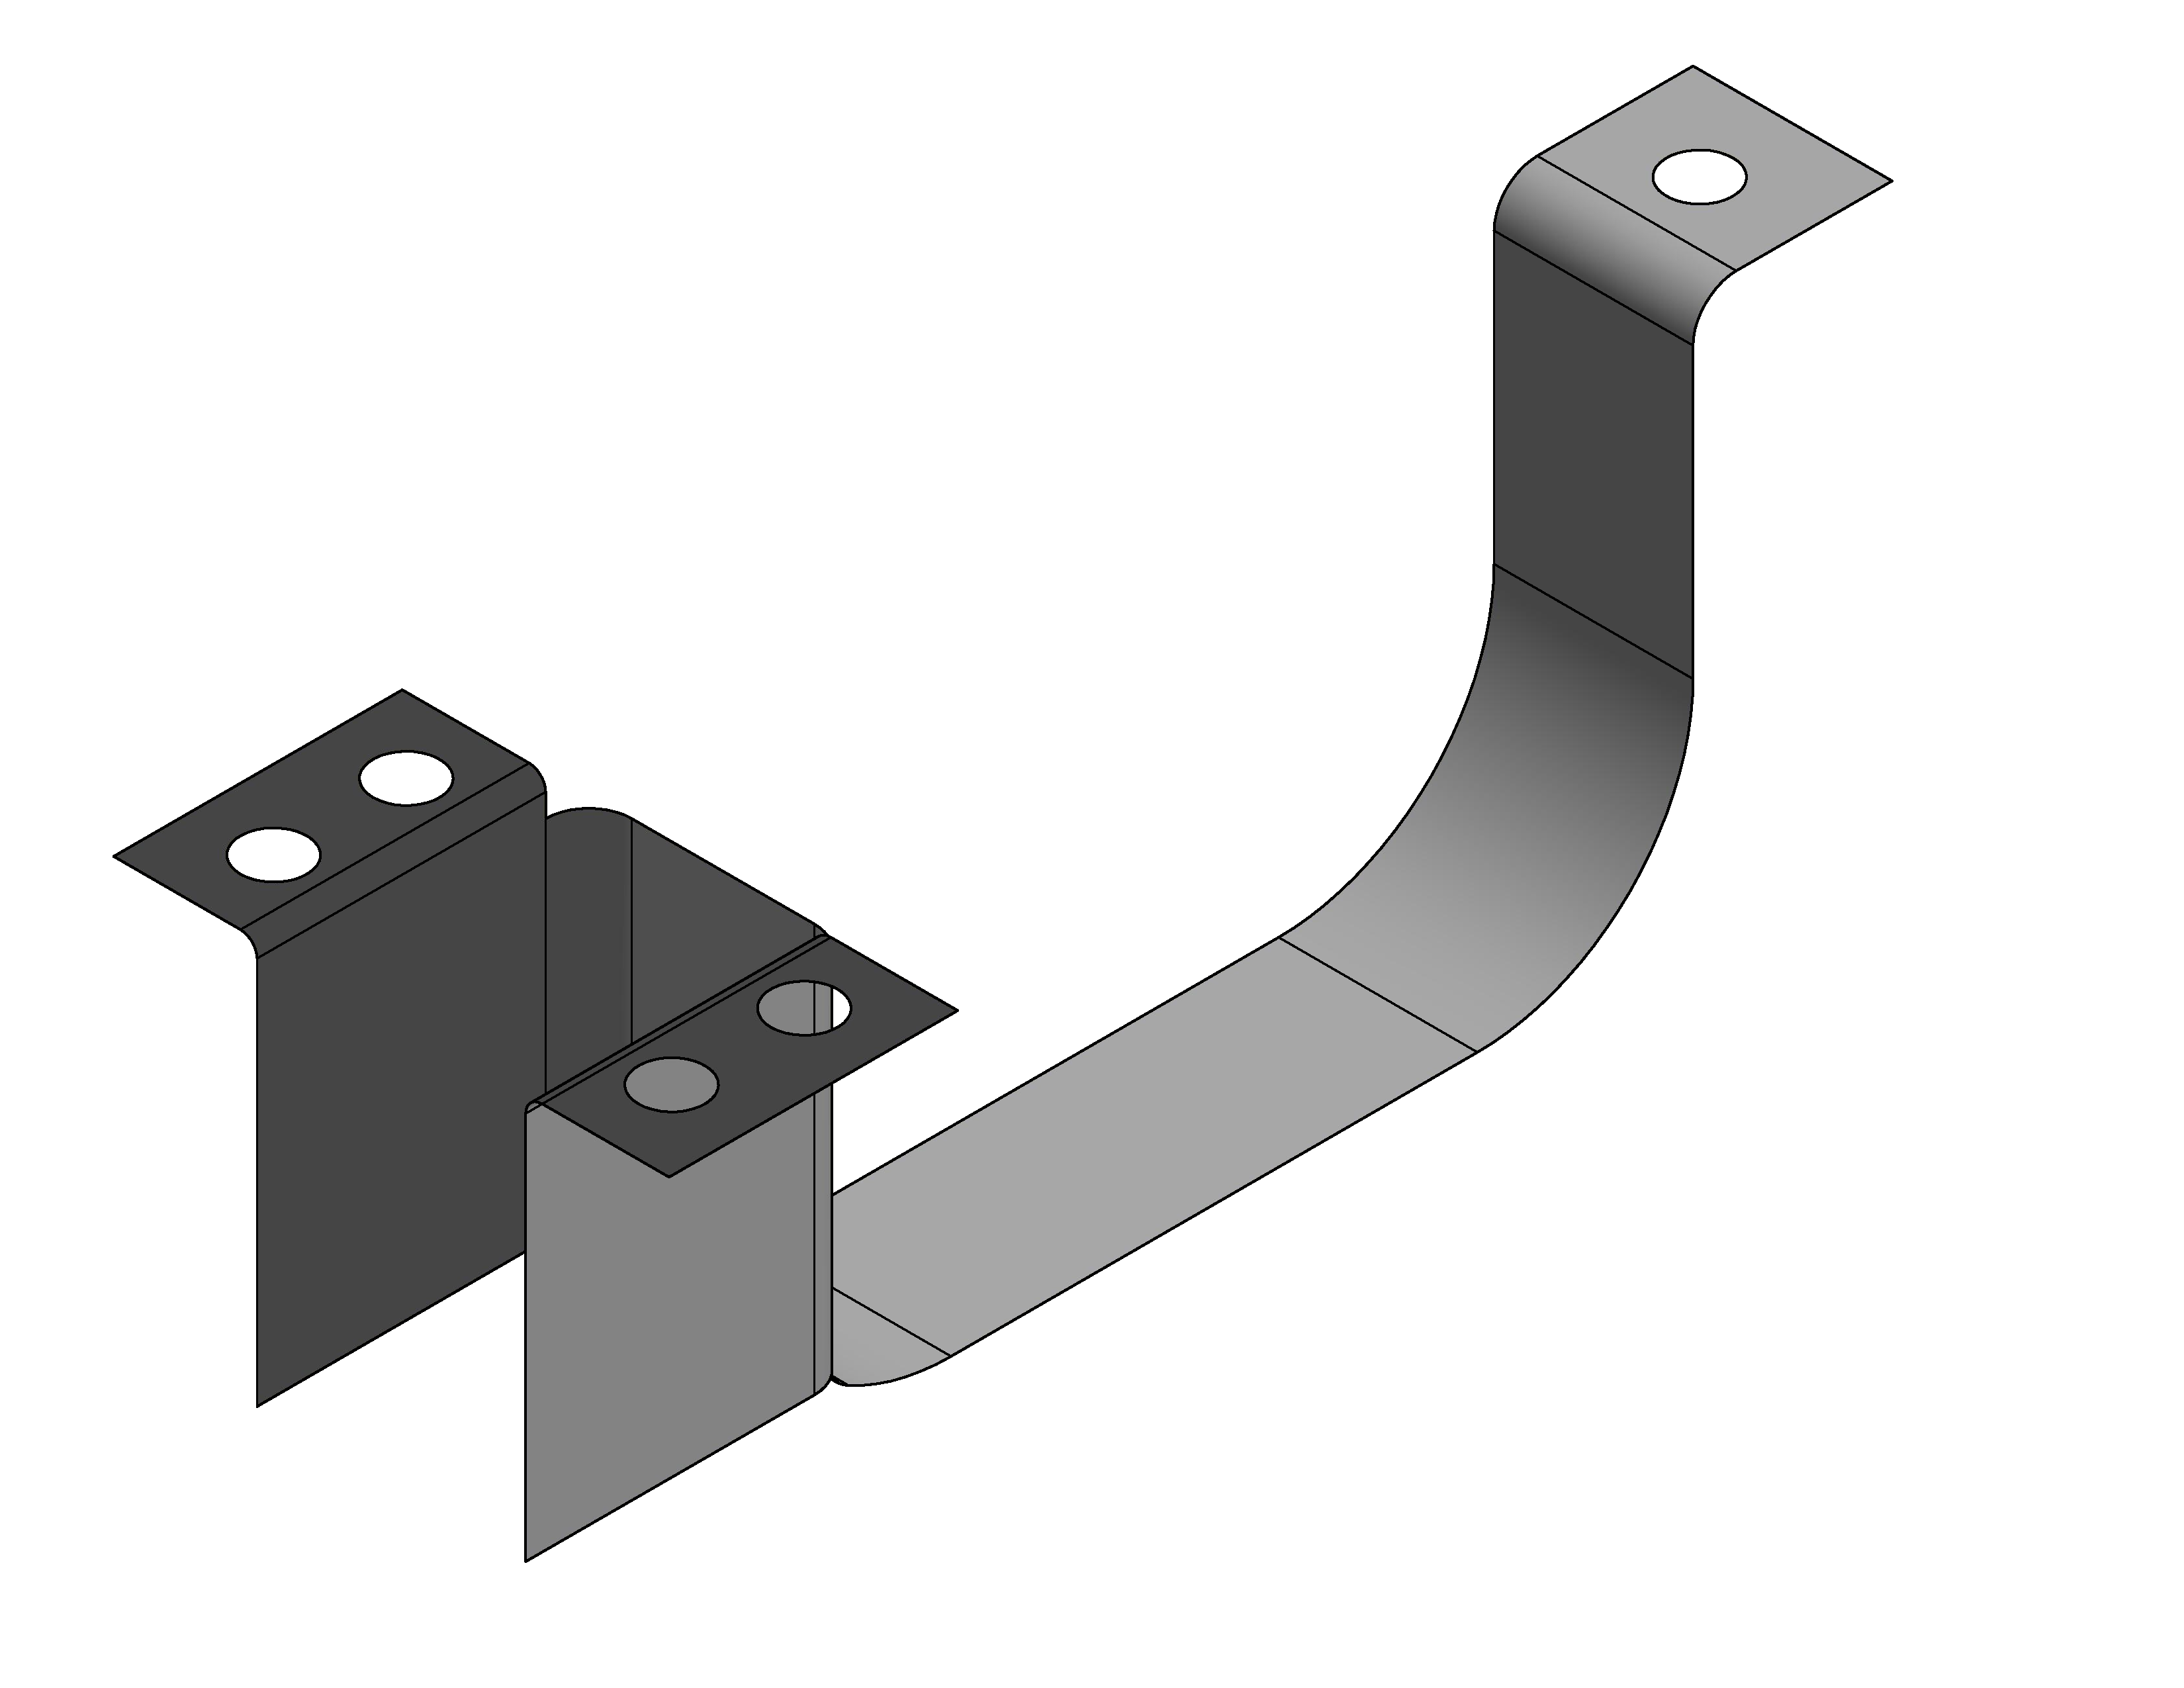
\includegraphics[width=\linewidth]{../Common/images/SimpleBracketMidsurfshaded.pdf} &
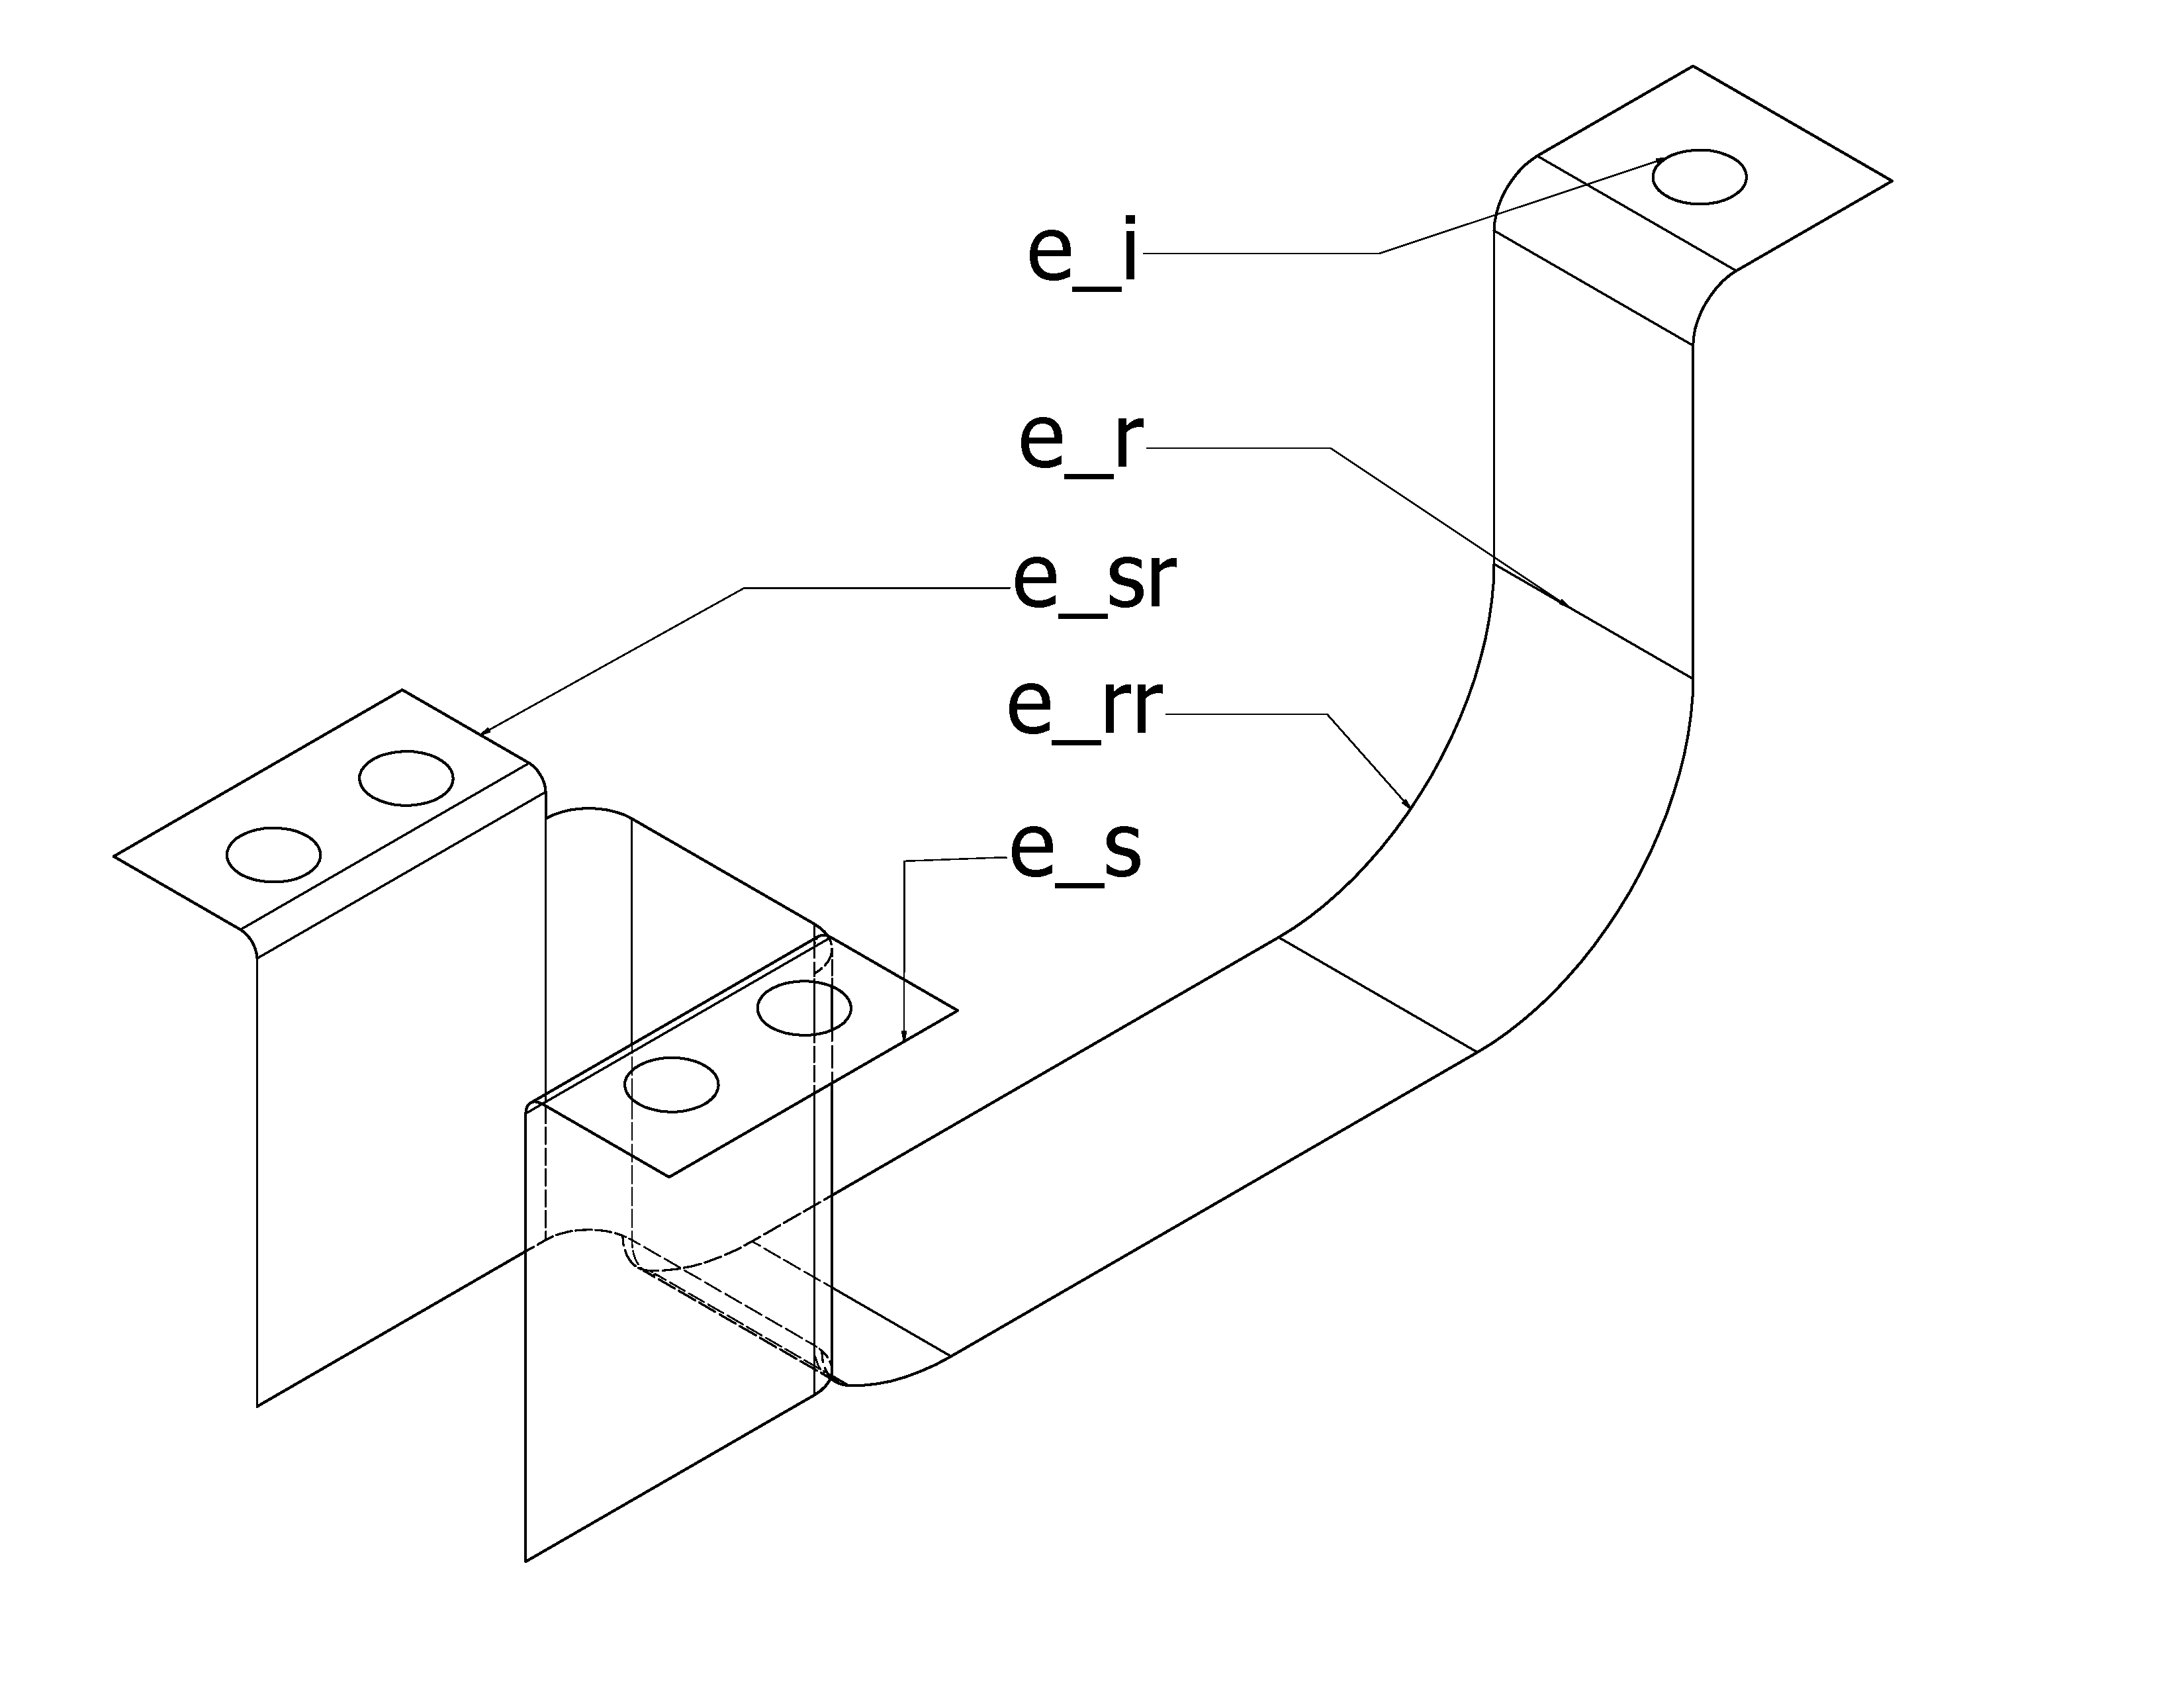
\includegraphics[width=\linewidth]{../Common/images/SimpleBracketMidsurf.pdf}\\
\end{tabular}

\begin{enumerate}
[noitemsep,topsep=2pt,parsep=2pt,partopsep=2pt,label=\textbullet]
\item Midsurface entities: \\$f = 15, e_s = 3, e_{sr} = 10, e_r = 14, e_{rr} = 19, l_p = 9 ,e_i=5,v_s = 8,v_r =24, v_i= 5, s=1,h=5,r=5$
\item Predicted solid-faces: \\$f_m = 2f+e_s+ l_p +e_i $\\$= 2 \times 15 + 3 + 9 + 5 = 47$
\item Predicted solid-edges: \\ $e_m = 2(e_s+e_{sr}+e_{rr}+e_i )+ \sum n_{r} e_{r}+v_s+v_i $\\$= 2(3+10+19 + 5)+ (2\times 12 + 4 \times 2)+8+5 = 119$
\item Predicted solid-vertices: \\$v_m = 2(v_s+ v_i) + \sum n_{r} v_r$\\$=2\times (8 + 5)  + 2 \times 24=74$
\item Predicted solid-shells-holes: \\$s_m =s = 1, h_m = r_i  = 5, r_m = 2r_i = 10$
\item Non-manifold equation of the left side  $\chi_{nml} $\\$= v-e+f $\\$= 32-46+15 = 1$
\item Non-manifold equation of the  right side  $\chi_{nmr}$\\$=s-h+r$\\$=1-5+5 = 1$
\item Manifold equation of the  left side  $\chi_{ml} $\\$= v_m-e_m+f_m $\\$=74-119+47= 2$
\item Manifold equation of the  right side  $\chi_{mr}$\\$=2(s_m-h_m )+r_m$\\$= 2(1-5)+10 = 2$
%\item Sheet metal midsurface characteristic $\chi_{smm}$\\$=
%e_s+e_i+(2-n_{r} ) e_{r}+e_{sr}/n_{r} $\\$=v_s+(2-n_{r} ) v_{r}+v_i$\\$ 4+0+0+0=4+0+0= 4$
%\item \textbf{Result}: \textcolor{green}{Matches}
\end{enumerate}
It can be observed that the predicted solid entities validate the manifold equation ($\chi_{ml} = \chi_{mr} = 2$). Validation can also be performed by comparing the  topological entities of the thin-walled solid with the predicted ones.
%----------------------------------------------------------------------------------------
%\item Closed Box of Surfaces  (Table \ref{table_TopoValClosedBox})
%
%\vspace{2mm}
%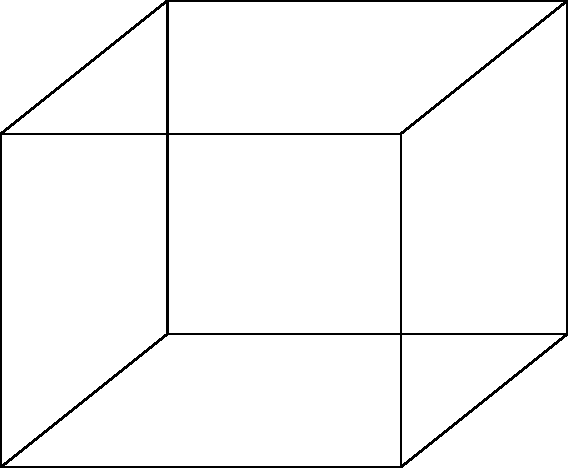
\includegraphics[width=0.6\linewidth]{../Common/images/ClosedBox.pdf} 
%\vspace{2mm}
%
%%----------------------------------------------------------------------------------------
%\begin{table}
%\caption{Closed Box of Surfaces}
%\begin{tabular}[t]{@{} p{0.035\linewidth}  p{0.035\linewidth} |  p{0.035\linewidth}  p{0.47\linewidth}  p{0.23\linewidth}@{}} \toprule
%{\bf NM } & {\bf \# }  & {\bf M} & {\bf Conversion } & {\bf Solid \# }  \\
%\midrule
%
%$f$ &
%$6$ &
%$f_m$ &
%$2f+e_s+e_{sr}/n_{r} +e_i $ &
%$12$\\
%
%$e_s$ &
%$0$ &
%$e_m$&
%$2(e_s+e_{sr}+e_i )+n_{r} e_{r}+v_s+v_i $&
%$24$\\
%
%$e_{sr}$&
%$0$&
%$v_m$&
%$2v_s+n_{r} v_r+2v_i $&
%$16$\\
%
%$e_r$&
%$12$&
%$s_m$&
%$s $&
%$2$\\
%
%$e_i$&
%$0$&
%$h_m$&
%$r_i $&
%$0$\\
%
%$v_s$&
%$0$&
%$r_m$&
%$2r_i $&
%$0$\\
%
%$v_r$&
%$8$&
%&
%NM Characteristic left side  $\chi_{nm-left}$ &
%$8-12+6=2$\\
%
%$v_i$&
%$0$&
%&
%NM Characteristic right side  $\chi_{nm-right}$ &
%$2-0+0=2$\\
%
%$s$&
%$2$&
%&
%M Characteristic left side  $\chi_{nm-left}$ &
%$16-24+12=4$\\
%
%$h$&
%$0$&
%&
%M Characteristic right side  $\chi_{nm-right}$ &
%$4$\\
%
%$r$&
%$0$&
%&
%Sheet metal midsurface characteristic $\chi_{smm}$,
%$e_s+e_i+(2-n_{r} ) e_{r}+e_{sr}/n_{r} =v_s+(2-n_{r} ) v_{r}+v_i $ &
%
%$0$\\
%\bottomrule
%\end{tabular}
%\label{table_TopoValClosedBox}
%\end{table}
%----------------------------------------------------------------------------------------
%\end{enumerate}

